\newcommand{\docNome}{Piano di Progetto}                          % NOME DEL DOCUMENTO
\newcommand{\docVersione}{0.1.0}                 % INSERIRE VERSIONE IN FORMATO x.y.z
\newcommand{\docStatus}{in lavorazione}          % AGGIORNARE SOLO QUANDO APPROVATO
\newcommand{\docUso}{Esterno}                           % INTERNO O ESTERNO
\newcommand{\docDestinatari}{
      Gruppo Sweven Team\\ %aggiungere altri con & Nome\\
      & Prof. Tullio Vardanega\\
      & Prof. Riccardo Cardin\\
      & Azienda Imola Informatica
} 
\newcommand{\docNomeTeam}{Sweven Team}
\newcommand{\docRedattori}{ %aggiungere altri con & Nome\\
      Matteo Pillon\\
      & Irene Benetazzo\\
      &Pan Qi Fan Andrea\\
      & Samuele Rizzato\\
}
\newcommand{\docVerificatori}{
  Tommaso Berlaffa \\
  & Irene Benetazzo\\
}
\newcommand{\docApprovazione}{}
\newcommand{\glossario}[1]{\textit{#1}\textsubscript{\textit{G}}}
\documentclass[12pt, a4paper,table]{article}
\usepackage[T1]{fontenc}
\usepackage[utf8]{inputenc}
\usepackage{lastpage}
\usepackage{hyperref}
\usepackage{fancyhdr}
\usepackage{fancyvrb}
\usepackage{geometry}
\usepackage{xcolor}
\usepackage{array}
\usepackage{graphicx}
\usepackage{float}
\usepackage{charter}
\usepackage{eurosym}
\usepackage{pdflscape}
\usepackage{longtable}
\hypersetup{
pdfborder = {0 0 0}
}
\geometry{a4paper,top=3cm,bottom=3cm,left=2cm,right=2cm}
\title{\textsc{\docNome}}
\author{}
\date{}
\definecolor{footer-gray}{HTML}{808080}
\pagestyle{fancy}
\fancyhf{}
\rhead{\textcolor{footer-gray}{\docNome} }
\lhead{\textcolor{footer-gray}{Sweven Team}}
\fancyfoot{}
\cfoot{\textcolor{footer-gray}{Pagina \thepage  \hspace{1pt} di \pageref*{LastPage}} }
\setcounter{tocdepth}{5}	%aggiunge paragrafi e sottoparagrafi all'indice
\setcounter{secnumdepth}{5}	%aggiunge numero indicizazzione a paragrafi e sottoparagrafi
\renewcommand*\contentsname{Indice}

\begin{document}
\maketitle
	\vspace{-3em}
	\begin{center}
	
\includegraphics[scale=0.50]{images/logo.jpg} \\
	\vspace{2em}
	\huge \textsc{\docNomeTeam}\\
	\normalsize \href{mailto:swe7.team@gmail.com}{swe7.team@gmail.com}\\
	\vspace{2em}
	\begin{tabular}{r|l}
		\multicolumn{2}{c}{ \textsc{Informazioni sul documento} } \\
		\hline
		\textbf{Versione}     & \docVersione\\
		\textbf{Uso}          & \docUso\\
        \textbf{Destinatari}  & \docDestinatari\\
		\textbf{Stato}        & \docStatus\\
		\textbf{Redattori}    & \docRedattori\\
		\textbf{Verificatori} & \docVerificatori\\
		\textbf{Approvatori} & \docApprovazione\\
	\end{tabular}
	\end{center}
    \vspace{3em}
    \begin{center}
        \LARGE{\textbf{Sintesi}} 
    \end{center}
    \normalsize{Guida per l'utente del prodotto \glossario{Chatbot}.}
	\thispagestyle{empty}   
	\newpage
\section*{Diario delle modifiche}
	\begin{center}
	\renewcommand{\arraystretch}{1.8} %aumento ampiezza righe
	\begin{longtable}{ |c|c|p{8em}|c|m{5em}|m{6em}| }
	\hline
	\textbf{Versione} & \textbf{Data} & \textbf{Descrizione} &  \textbf{Ruolo} &  \textbf{Autore} & \textbf{Verificatore}\\ %Aggiungere le nuove righe sopra la prima
	\hline % Se il nome non ci sta, metterlo a mano con aggiunta di \newline (esempio: Nome \newline Cognome)
    & 2022-08-09 & Scrittura \$3 & Amministratore & Irene \newline Benetazzo & \\ 
	\hline
	& 2022-08-08 & Scrittura \$1 & Amministratore & Irene \newline Benetazzo & \\ 
	\hline
	& 2022-07-21 & Creazione documento & Amministratore & Irene \newline Benetazzo & \\ 
	\hline
	\end{longtable}
	\end{center}
	\newpage
\tableofcontents
\newpage
\section{Introduzione}
    \subsection{Scopo del Documento}
Il seguente documento è necessario per organizzare la suddivisione dei lavori all'interno del gruppo e la conseguente realizzazione del progetto. Per ogni attività verranno dunque definiti i seguenti attributi: 
\begin{itemize}
    \item Rischi connessi allo svolgimento dell'attività
    \item Attribuzione di un ruolo ad ogni membro del team per consentirne lo svolgimento
    \item Preventivo risorse necessarie per portarla a termine
    \item Tempo e risorse effettivamente impiegate per la realizzazione
    \item Analisi generale dell'attività svolta
\end{itemize}
La definizione di tali attributi permette di organizzare il lavoro in maniera efficiente in modo tale da consentire al gruppo di lavorare in parallelo. 

\subsection{Scopo del Capitolato}
Lo scopo di tale progetto è quello di sviluppare un Chatbot, che interfacciandosi con software aziendali, spesso complessi e dispersivi semplifichi i compiti che i dipendenti devono svolgere. In particolare vengono individuate le seguenti operazioni: 
\begin{itemize}
    \item Tracciamento della presenza in sede (\textbf{EMT}\textsubscript{G})
    \item Rendiconto attività svolte quotidianamente (\textbf{EMT}\textsubscript{G})
    \item Apertura del cancello aziendale (\textbf{MQTT}\textsubscript{G})
    \item Creazione di una riunione in un servizio esterno
    \item Servizio di ricerca documentale (\textbf{CMIS}\textsubscript{G})
    \item Creazione e tracciamento di bug (\textbf{Redmine}\textsubscript{G})
\end{itemize}

\subsection{Glossario}
Per assicurare la massima fruibilità e leggibilità del documento, il team SWEven ha deciso di creare un documento denominato \textit{Glossario} il cui scopo sarà quello di contenere le definizioni dei termini ambigui o specifici del progetto. Sarà possibile riconoscere i termini presenti al suo interno in quanto terminanti con la lettera \textit{G} posta come pedice della parola stessa. 
\subsection{Riferimenti}

\subsubsection{Normativi}
\begin{itemize}
    \item IEEE 830-1998 Specifica dei requisiti software
    \item Norme di progetto {\docVersionNdP}
    \item Verbale esterno 2022-03-18
    \item Verbale esterno 2022-04-15
\end{itemize}

\subsubsection{Informativi}
\begin{itemize}
    \item \href{https://www.math.unipd.it/~tullio/IS-1/2021/Progetto/C1.pdf}{\color{blue} Capitolato di appalto C1 - BOT4ME}
    \item \href{https://www.math.unipd.it/~tullio/IS-1/2021/Dispense/T07.pdf}{\color{blue} Slide del corso - Analisi dei requisiti}
    \item \href{https://www.math.unipd.it/~rcardin/swea/2022/Diagrammi%20Use%20Case.pdf}{\color{blue} Slide del corso - Diagrammi dei casi d'uso}
\end{itemize}
\newpage
\section{Analisi dei rischi}
      \subsection{Descrizone}
Durante lo svolgimento del progetto è inevitabile riscontrare vari problemi e imprevisti, quindi il gruppo ritiene opportuno svolgere l’attività dell’analisi dei rischi per evitare o mantenere al minimo i danni possibili.\newline
L’identificazione e la gestione dei rischi vengono effettuato nelle seguenti fase:
\begin{enumerate}
\item identificazione:  il gruppo identifica tutti i possibili rischi che possono danneggiare la qualità del lavoro;
\item aanalisi dei rischio: per ogni rischio individuare il suo livello di gravità e la possibile conseguenza;
\item pianificazione: vengono definite le precauzioni necessarie per evitare il rischio, e le azioni necessarie nel caso in cui il rischio avvenga;
\item controllo: monitorare continuo durante lo svolgimento dell’attività, agire di conseguenza.
\end{enumerate}

\subsection{Tipi di rischi}
Il gruppo individua quattro tipologie di rischi principali:
\begin{itemize}
\item rischi tecnologiche;
\item rischi personali;
\item rischi organizzativi;
\item rischi per requisiti.
\end{itemize}

\subsection{Elenchi dei rischi}
In questo capitolo vengono riportati quattro elenchi di rischi divisi per tipologia che il gruppo ha attualmente individuato.
Per ogni rischio viene assegnato un codice di riferimento, la gravità valutato dal gruppo, la sua conseguenza, le precauzioni necessarie e le contromisure da applicare nel momento in cui il rischio accade. 
\subsubsection{Rischi tecnologiche}
\textbf RT1:
 Ritardo dovuto all'uso delle nuove tecnologie
\begin{itemize}
\item Livello di gravità: 2;
\item Conseguenze: maggior tempo di apprendimento;
\item Precauzioni: ogni membro si impegna continuamente a comunicare il progresso della propria attività, in caso di difficoltà comunica al gruppo durante e non al termine della scadenza, per cercare un aiuta da parte del gruppo;
\item Contromisure: per ogni nuove tecnologie usata, si cerca di capire la complessità a priori, e di stabilire le tempistiche più lasche valutando la difficoltà della tecnologia.
\end{itemize}

\textbf RT2: 
Perdita di dati dovuti al malfunzionamento del hardware
\begin{itemize}
\item Livello d gravità: 2;
\item Conseguenze: una parte del lavoro viene perso completamente, tutti i lavori dipendenti da questo lavoro vengono ritardati, può causare un effetto collaterale;
\item Precauzioni: tutti i lavori completati devono essere salvati nello strumento condiviso, ogni membro si impegna a salvare il proprio lavoro in corso frequentemente in un dispositivo alternativo;
\item Contromisure: il componente si impegna a recuperare velocemente il lavoro perso, il responsabile si occupa di riassegnare i task al resto del componente.
\end{itemize}

\textbf RT3: 
Tecnologia non utilizzabile dovuto alla mancanza dei requisiti o alla complessità
\begin{itemize}
\item Livello d gravità: 1;
\item Conseguenze: può causere una piccola perdita di tempo di lavoro;
\item Precauzioni: nei confronti delle nuove tecnologie, l'analista deve sempre fare una ricerca a priori per valutare l'utilizzabilità;
\item Contromisure: il gruppo dovrà rivalutare un possibile sostituto velocemente.
\end{itemize}

\subsubsection{Rischi personali}
\textbf RP1: 
Contrasto fra i membri
\begin{itemize}
\item Livello di gravità: 3;
\item Conseguenze: possibili ritardi dei lavori per il mancato collaborazione;
\item Precauzioni: tutti i membri devono portare rispetto per gli altri, usando un linguaggio lecito ed educato;
\item Contromisure: il responsabile deve riassegnare il lavoro, evitando che il problema peggiorasse, in seguito cercare una soluzione con il team.
\end{itemize}
\textbf RP2:
Mancato consegna del task assegnato
\begin{itemize}
\item Livello di gravità: 2;
\item Conseguenza: interrompe il normale flusso di lavoro progettato;
\item Precauzioni: prima di assegnare un task, esso deve essere analizzato la sua complessità, ogni membro deve essere assegnato un task fattibile nell'arco di tempo dedicato;
\item Contromisure: il soggetto deve comunicare al responsabile il motivo della mancanza, eventualmente il responsabile riassegna il task suddiviso agli altri membri del gruppo.
\end{itemize}

\subsubsection{Rischi organizzativi}
\textbf RO1: 
iìImpegno organizzativi dovuto ai problemi accademici o di lavoro
\begin{itemize}
\item Livello di gravità: 1;
\item Conseguenze: indisponibilità di qualche unione o attività per un certo periodo;
\item Precauzioni: ogni membro deve comunicare al gruppo i propri impegni personali, il responsabile deve assegnare i task in base alla disponibilità indicata;
\item Contromisure: al momento in cui un membro del gruppo non avesse la disponibilità a causa di un problema provvisorio, comunica immediatamente al responsabile, il responsabile riassegna i task agli altri membri oppure prolungare il tempo progettato per quel task.
\end{itemize}

\subsubsection{Rischi per requisiti}
\textbf RR1: 
Errata comprensione dei requisiti
\begin{itemize}
\item Livello di gravità: 4;
\item Conseguenze: nel peggior caso, può richiedere una ristrutturazione notevole del lavoro svolto;
\item Precauzioni: durante la progettazione e lo sviluppo, scambiare spesso l’informazione con l’azienda, se necessario, chiedere un unione per chiarire domande non chiare;
\item Contromisure: evitare sempre.
\end{itemize}
\textbf RR2:
Cambiamento dei requisiti
\begin{itemize}
\item Livello di gravità: 5;
\item Conseguenza: puo causare un enorme ristrutturazione del lavoro;
\item Precauzioni: un dialogo frequente con l'azienda per essere aggiornato ad ogni momento;
\item Contromisure: il responsabile deve subito chiedere una riuniune interna, valutare con il gruppo i cambiamenti neccessati, ripianificare subito il lavoro quando dovesse.
\end{itemize}




\section{Modello di sviluppo}
      \subsection{Descrizione}
Data la scarsa esperienza pregressa da parte dei componenti del gruppo nella gestione di un progetto, si è deciso di gestire l'organizzazione nella maniera più efficacie ed efficiente possibile adottando un modello \glossario{agile} per lo sviluppo del progetto. In particolare si è deciso di seguire le linee guida del modello incrementale, il quale facilita l'analisi e la stesura dei requisiti. 
\subsection{Modello Incrementale}
Il modello incrementale prevede una serie di rilasci multipli e successivi, ciascuno dei quali è costituito dai seguenti passi: 
\begin{itemize}
    \item analisi requisiti;
    \item implementazione;
    \item test;
    \item valutazione.
\end{itemize}
\subsubsection{Vantaggi del Modello Incrementale}
L'adozione di un modello ciclico come quello incrementale permette di usufruire di una serie di vantaggi: 
\begin{itemize}
    \item ogni incremento permette di avere indicazioni utili all'incremento successivo;
    \item il rischio di fallimento viene ridotto ad ogni incremento;
    \item gli errori vengono limitati in quanto la possibilità che si verifichino è limitata all'interno del singolo incremento, infatti al termine dello stesso segue una fase di verifica;
    \item le funzionalità primarie hanno priorità più elevata permettendo di avere fin da subito un prototipo funzionante che il proponente può valutare.
\end{itemize}
\newpage
\section{Pianificazione}
      \subsection{Introduzione}
Il gruppo Sweven ha deciso di suddividere il lavoro in macrofasi seguendo le revisioni da effettuare con il committente:
\begin{itemize}
    \item \textbf{RTB:} Requirements Technology Baseline è prevista per fine Maggio 2022
    \item \textbf{PB:} Product Baseline prevista nel mese di Agosto 2022
    \item \textbf{CA:} Customer Acceptance prevista nel mese di Settembre 2022
\end{itemize}

\subsubsection{Diagramma di Gantt}
Nel diagramma di Gantt le varie attività vengono riportate mediante una dicitura sintetica. 
I colori indicano la tipologia dell'attività o la priorità di essa rispetto alle altre della stessa fase:
\begin{itemize}
    \item \textbf{Nero:} indica il periodo dell'intera fase;
    \item \textbf{\textcolor{red}{Rosso:}} indica attività con priorità alta;
    \item \textbf{\textcolor{violet}{Viola:}} indica attività con priorità media;
    \item \textbf{\textcolor{cyan}{Azzurro:}} indica attività da mantenere aggiornata o fare se necessaria in relazione alle altre attività;
    \item \textbf{\textcolor{yellow}{Giallo:}} verifica delle attività eseguite durante la fase;
    \item \textbf{\textcolor{green}{Verde:}} approvazione di ciò che è stato fatto finora (non solo durante la fase stessa);
    \item \textbf{\textcolor{blue}{Blù:}} attività di consuntivazione delle ore e del costo;
    \item \textbf{\textcolor{orange}{Arancione:}} indica preparazione per la revisione .
\end{itemize}

\subsubsection{Checkpoint}
Al termine di ogni fase è prevista una riunione interna di tutti i membri del gruppo:
    \begin{itemize}
        \item rendicontazione delle ore effettivamente necessarie per i task assegnati:
        \item analisi rispetto alla pianificazione e preventivo costi;
        \item analisi di eventuali criticità;
        \item valutazione di eventuali modifiche sulla pianificazione futura;
        \item organizzazione nel dettaglio, assegnando i singoli task per la fase successiva. 
    \end{itemize}

      \subsection{Requirements Technology Baseline}
Questa macrofase è suddivisa in tre fasi:
\begin{itemize}
    \item \textbf{Baseline documentale} dal 2022-04-19 al 2022-05-02;
    \item \textbf{Baseline dei requisiti} dal 2022-05-03 al 2022-05-09;
    \item \textbf{Baseline delle tecnologie} dal 2022-05-10 al 2022-05-23.
\end{itemize}

\subsubsection{Baseline documentale}
\begin{itemize}
    \item \textbf{Norme di Progetto:} l'amministratore redige le norme e gli strumenti necessari ad una buona organizzazione e realizzazione del progetto;
    \item \textbf{Piano di Progetto:} l'analista rileva i possibili rischi che possono sorgere durante il progetto, il responsabile pianifica la macrofase RTB;
    \item \textbf{Piano di Qualifica:} l'analista stabilisce e redige i parametri di qualità stabilendo soglie minime accettabili e soglie desiderate; 
    \item \textbf{Glossario:} viene aggiornato se ritenuto necessario durante altre attività;
    \item \textbf{Verifica:} il verificatore controlla che siano state rispettate le norme e verifica il materiale scritto durante questa fase;
    \item \textbf{Checkpoint:} per la descrizione dettagliata si veda \$4.1.2 . 
\end{itemize}

\subsubsection{Baseline dei requisiti}
\begin{itemize}
    \item \textbf{Analisi dei Requisiti:} l'analista studia e descrive tutti i requisiti del progetto commissionato dal proponente, 
                comprese tutte le richieste opzionali e desiderabili (indipendentemente dalla possibilità di realizzarle tutte);
    \item \textbf{Norme di Progetto, Piano di Progetto, Piano di Qualifica:} documenti che vengono incrementati e aggiornati;
    \item \textbf{Glossario:} viene aggiornato se ritenuto necessario durante altre attività;
    \item \textbf{Verifica:} il verificatore controlla che siano state rispettate le norme e verifica il materiale scritto prodotto durante questa fase;
    \item \textbf{Checkpoint:} per la descrizione dettagliata si veda \$4.1.2 .
\end{itemize}

\subsubsection{Baseline delle tecnologie}
\begin{itemize}
    \item \textbf{Specifica Architetturale:} il progettista, analizzando lati positivi e negativi, sceglie le tecnologie per il progetto, assegnando poi lo studio autonomo al gruppo.
    \item \textbf{Proof of Concept:} il progettista implementa la dimostrazione del progetto integrando le varie tecnologie e alcune funzionalità principali.
    \item \textbf{Norme di Progetto, Piano di Progetto, Piano di Qualifica:} documenti che vengono incrementati e aggiornati;
    \item \textbf{Glossario:} viene aggiornato se ritenuto necessario durante altre attività;
    \item \textbf{Verifica:} il verificatore controlla che siano state rispettate le norme e verifica il materiale scritto e il prodotto realizzato durante questa fase;
    \item \textbf{Approvazione:} il responsabile controlla, approva il materiale e il prodotto realizzato durante questa macrofase;
    \item \textbf{Checkpoint:} per la descrizione dettagliata si veda \$4.1.2;
    \item \textbf{Presentazione RTB:} viene preparata la presentazione per il colloquio e pubblicato il materiale nella repository pubblica.
\end{itemize}


\begin{landscape}
	\begin{figure}
	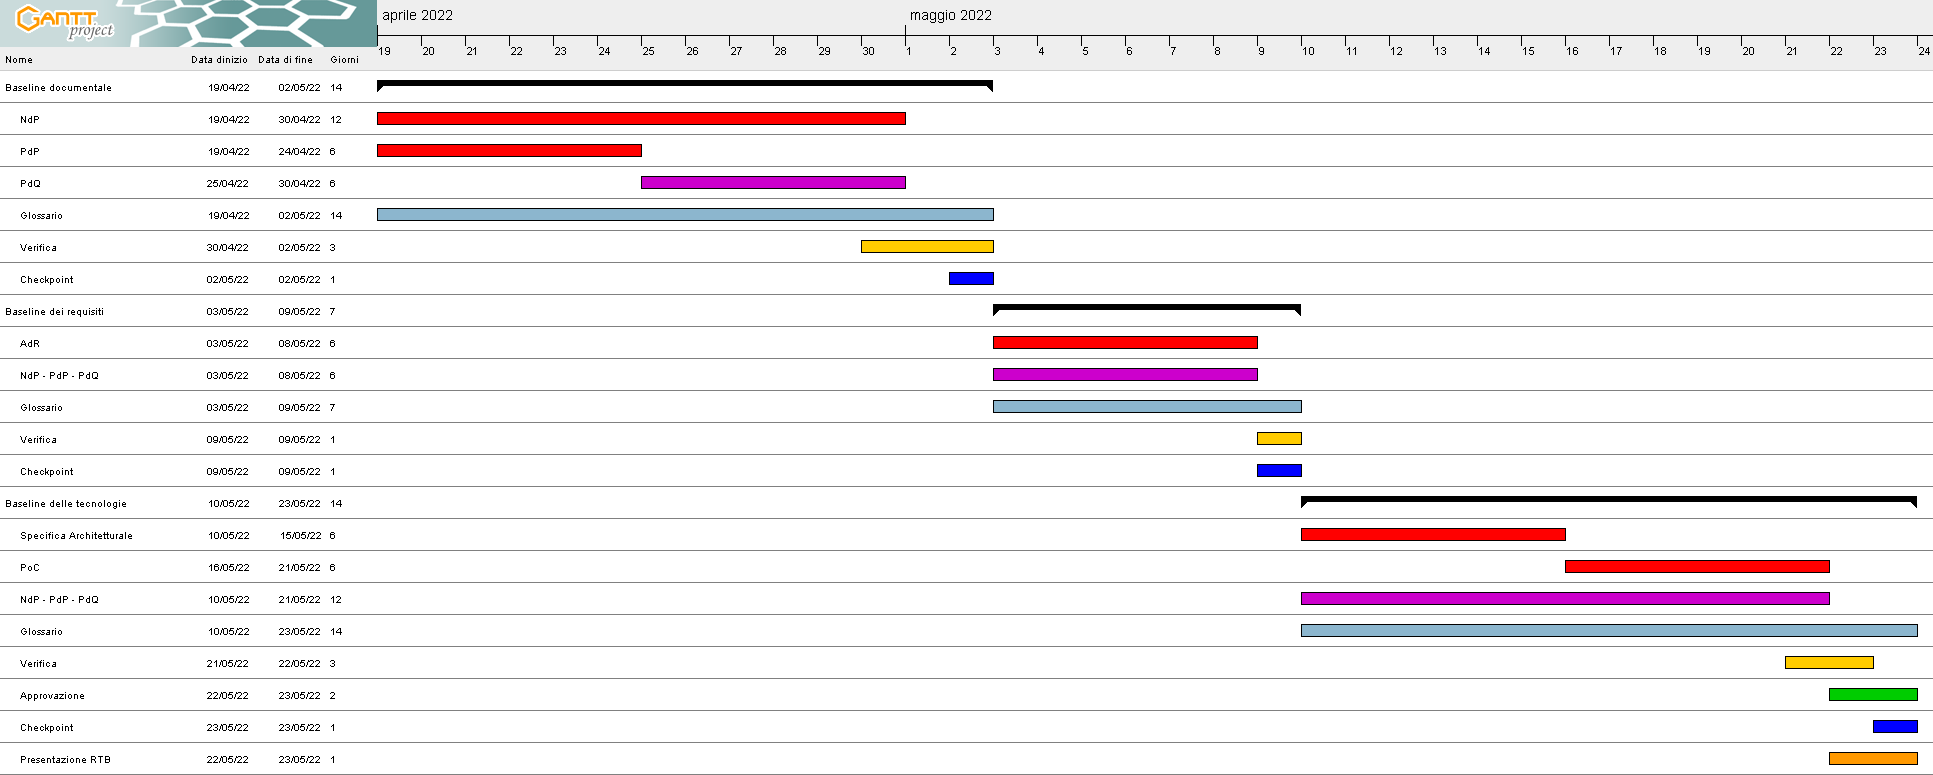
\includegraphics[width=\linewidth]{images/preventivo/RTB-Gantt.png}
    \caption{Diagramma di Gantt - Macrofase RTB}
	\end{figure}
\end{landscape}
      \subsection*{Periodo per eventuale recupero e revisione}
Dal 24 Maggio al 13 Giugno si prevedono giorni di recupero per terminare la macrofase RTB e i giorni necessari ad effettuare il colloquio con i committenti.

\subsection{Product Baseline}
La macrofase Product Baseline è suddivisa in 4 incrementi che sono raggruppati in 2 fasi:
\begin{itemize}
    \item \textbf{Requisiti Obbligatori} dal 2022-06-13 al 2022-07-11;
            \begin{itemize}
                \item Incremento 1 dal 2022-06-13 al 2022-06-27;
                \item Incremento 2 dal 2022-06-28 al 2022-07-11;
            \end{itemize}
    \item \textbf{Requisiti Desiderabili} dal 2022-07-12 al 2022-07-25;
            \begin{itemize}
                \item Incremento 3 dal 2022-07-12 al 2022-07-18;
                \item Incremento 4 dal 2022-07-19 al 2022-07-25;
            \end{itemize}
\end{itemize}
Per la descrizione, corrispondenza tra i codici dei casi d'uso e i requisiti si faccia riferimento al documento Analisi dei Requisiti {\docVersionAdR}. \newline
Per ogni implementazione di una funzionalità il progettista progetta, il programmatore scrive il codice implementandola e il verificatore esegue i test di controllo segnalando gli eventuali errori / bug.
\subsubsection{Requisiti Obbligatori}
\paragraph{Incremento 1}
\begin{itemize}
    \item \textbf{Implementazione input testuale e vocale:} RO-F-1, 2, 61;
    \item \textbf{Implementazione autenticazione mediante \glossario{token}:} RO-F-3 a 6, 51, 52, 57 (UC1, UC13, UC18);
    \item \textbf{Implementazione gestione comandi non validi ed errori:} RO-F-8, 9, da 47 a 50 (UC2, UC10, UC11, UC12);
    \item \textbf{Specifica Architetturale, Manuale Utente:} creazione e inizio scrittura dei documenti con progettista e programmatore. La Specifica Architetturale illustrerà l'architettura del prodotto, mentre il Manuale Utente fornirà le istruzioni necessarie per l'uso del \glossario{chatbot};
    \item \textbf{Verifica:} il verificatore controlla che siano state rispettate le norme e verifica il materiale scritto e il prodotto realizzato durante questa fase;
    \item \textbf{Checkpoint:} per la descrizione dettagliata si veda \$4.1.2;
\end{itemize}

\paragraph{Incremento 2}
\begin{itemize}
    \item \textbf{Implementazione della registrazione presenza:} RO-F-10 a 12, 46, 60 (UC3, UC9, UC20);
    \item \textbf{Implementazione della consuntivazione:} RO-F-13 a 21, 53, 54, 62 (UC4, UC14, UC15, UC21);
    \item \textbf{Specifica Architetturale, Manuale Utente:} continua la scrittura dei documenti con progettista e programmatore;
    \item \textbf{Verifica:} il verificatore controlla che siano state rispettate le norme e verifica il materiale scritto e il prodotto realizzato durante questa fase;
    \item \textbf{Checkpoint:} per la descrizione dettagliata si veda \$4.1.2;
\end{itemize}

\begin{landscape}
	\begin{figure}
	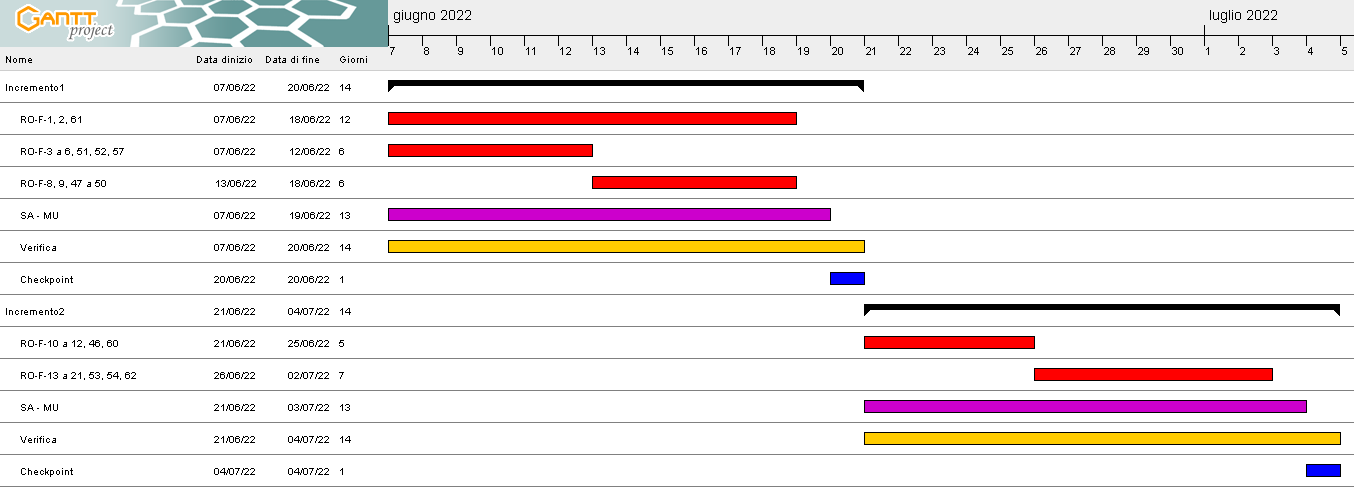
\includegraphics[width=\linewidth]{images/PB_obbligatori.png}
    \caption{Diagramma di Gantt - Macrofase PB, fase Requisiti Obbligatori}
	\end{figure}
\end{landscape}

\subsubsection{Requisiti Desiderabili}
\paragraph{Incremento 3}
\begin{itemize}
    \item \textbf{Implementazione autenticazione a scelta tra più \glossario{token}:} RD-F-7;
    \item \textbf{Implementazione della creazione di riunioni:} RD-F-24 a 32, 56, 58, 59 (UC6, UC17, UC19);
    \item \textbf{Implementazione dell'apertura del cancello:} RO-F-22, 23 (UC5);
    \item \textbf{Specifica Architetturale, Manuale Utente:} continua la scrittura dei documenti con progettista e programmatore;
    \item \textbf{Verifica:} il verificatore controlla che siano state rispettate le norme e verifica il materiale scritto e il prodotto realizzato durante questa fase;
    \item \textbf{Checkpoint:} per la descrizione dettagliata si veda \$4.1.2;
\end{itemize}

\paragraph{Incremento 4}
\begin{itemize}
    \item \textbf{Implementazione della ricerca di documenti:} RO-F-33 a 37, 55 (UC7, UC16);
    \item \textbf{Implementazione dell'inserimento di \glossario{ticket}:} RO-F-38 a 45 (UC8);
    \item \textbf{Specifica Architetturale, Manuale Utente:} termina la scrittura dei documenti;
    \item \textbf{Verifica:} il verificatore controlla che siano state rispettate le norme e verifica il materiale scritto e il prodotto realizzato durante questa fase;
    \item \textbf{Approvazione:} il responsabile controlla, approva il materiale e il prodotto realizzato durante questa macrofase PB;
    \item \textbf{Checkpoint:} per la descrizione dettagliata si veda \$4.1.2;
    \item \textbf{Presentazione PB:} viene preparata la presentazione per il colloquio e pubblicato il materiale nella repository pubblica e nel branch main.
\end{itemize}

\begin{landscape}
	\begin{figure}
	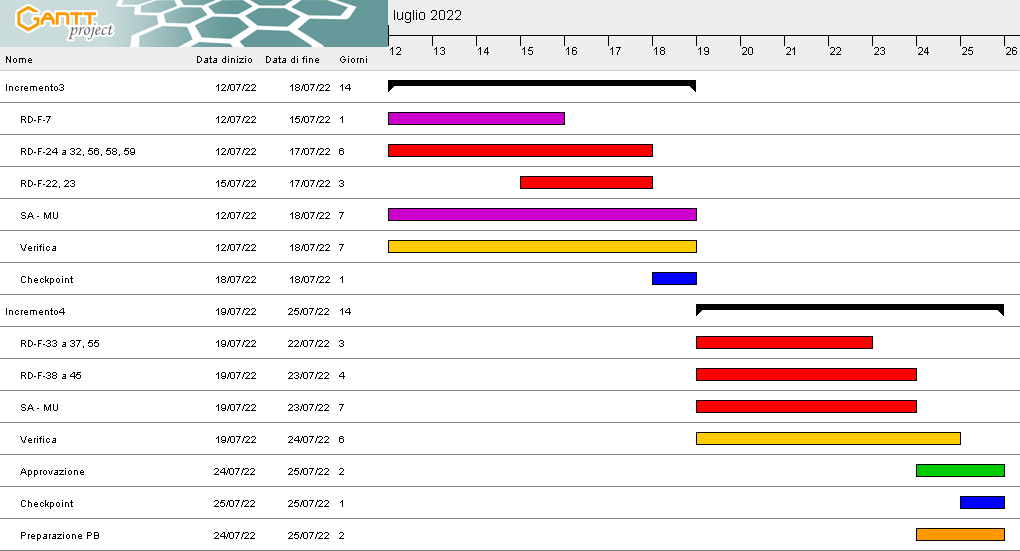
\includegraphics[width=\linewidth]{images/PB_desiderabili.png}
    \caption{Diagramma di Gantt - Macrofase PB, fase Requisiti Desiderabili}
	\end{figure}
\end{landscape}

\begin{landscape}
	\begin{figure}
	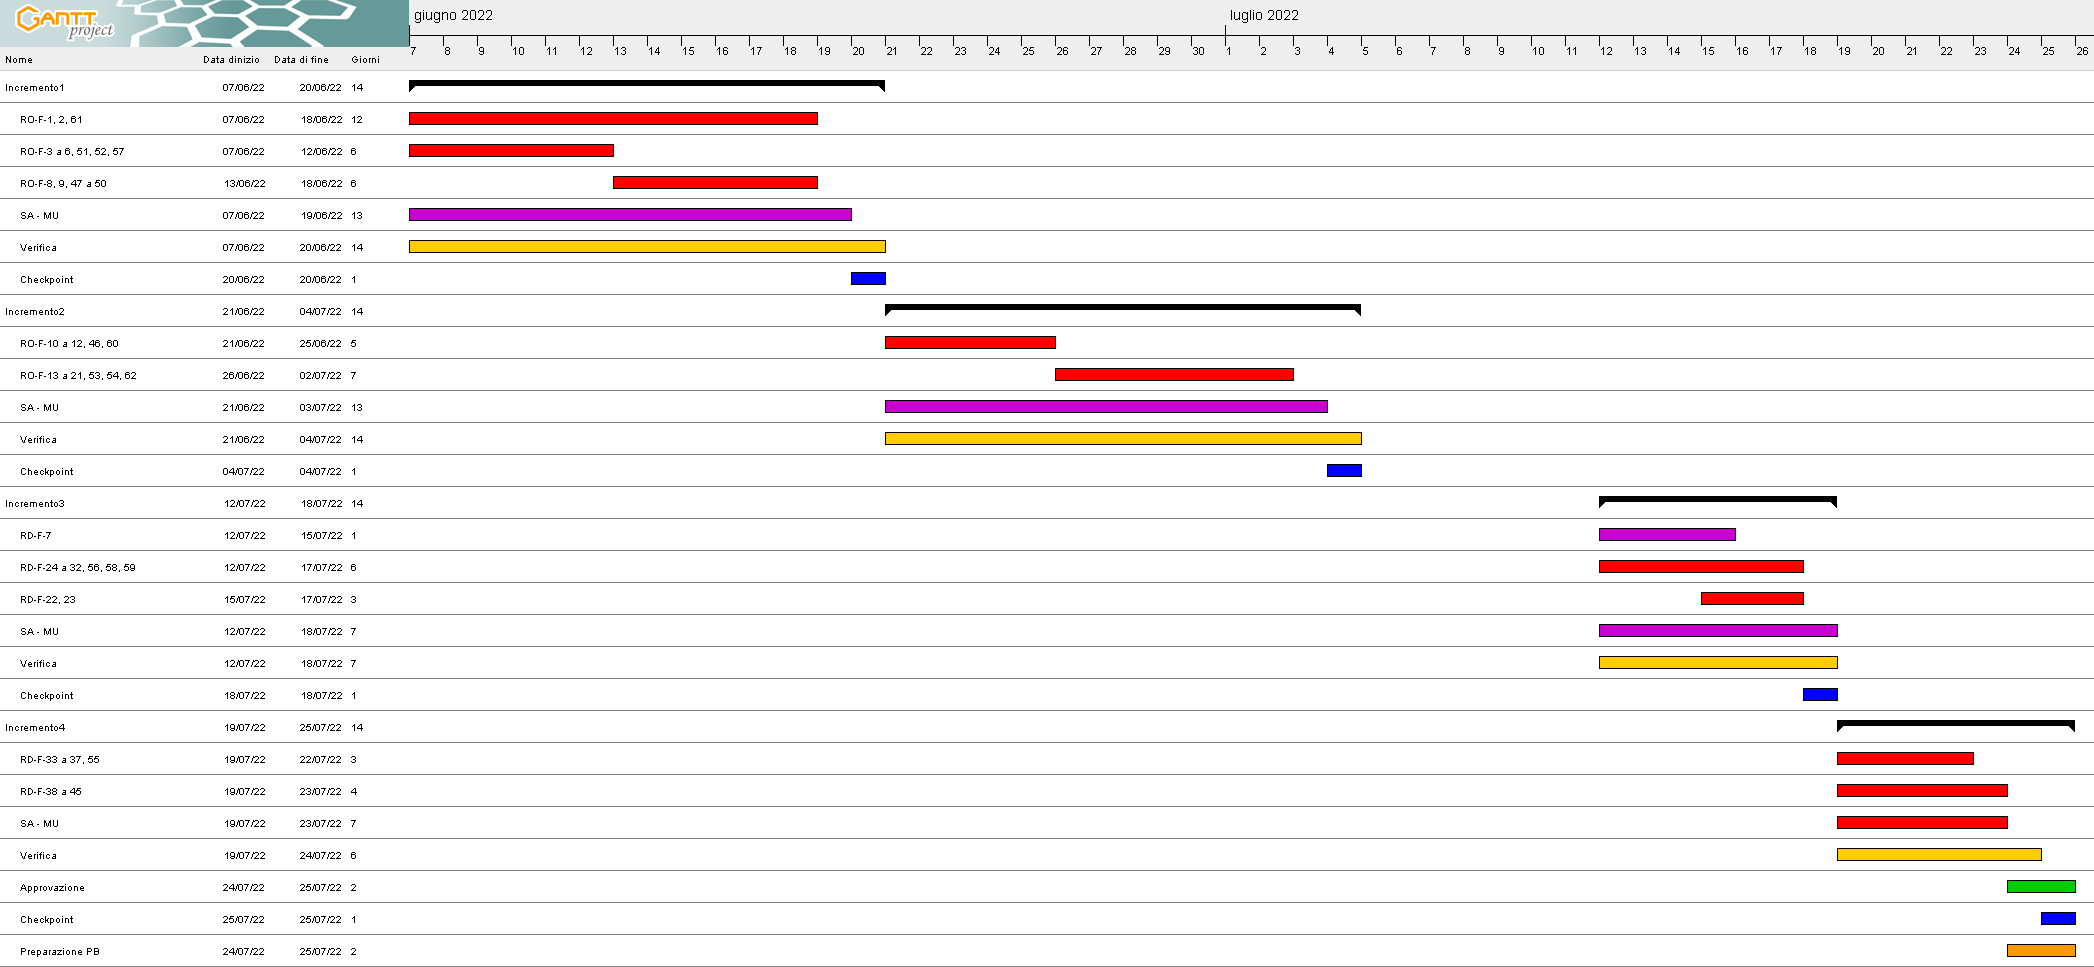
\includegraphics[width=\linewidth]{images/PB.png}
    \caption{Diagramma di Gantt - Macrofase PB}
	\end{figure}
\end{landscape}

\newpage
      \subsection{Customer Acceptance}
Per la macrofase Customer Acceptance sono previste 2 fasi da una settimana ciascuna:
\begin{itemize}
    \item Validazione requisiti obbligatori dal 2022-09-12 al 2022-09-19
    \item Validazione requisiti desiderabili dal 2022-09-20 al 2022-09-26
\end{itemize}
\subsubsection{Validazione requisiti obbligatori}
\begin{itemize}
    \item \textbf{Implementazione di test:} principalmente test di sistema;
    \item \textbf{Validazione e collaudo:} dei requisiti obbligatori;
    \item \textbf{Opzionale:} implementazione funzionalità creazione riunione;
    \item \textbf{Checkpoint:} per la descrizione dettagliata si veda \$4.1.2
\end{itemize}
\subsubsection{Validazione requisiti desiderabili}
\begin{itemize}
    \item \textbf{Validazione e collaudo:} dei requisiti facoltativi;
    \item \textbf{Approvazione:} il responsabile controlla, approva quanto realizzato in questa macrofase;
    \item \textbf{Checkpoint:} per la descrizione dettagliata si veda \$4.1.2
    \item \textbf{Presentazione CA:} viene effettuato il release del prodotto e di tutti i documenti. Viene preparata la presentazione per il colloquio finale.
\end{itemize}
\begin{figure}[H]
	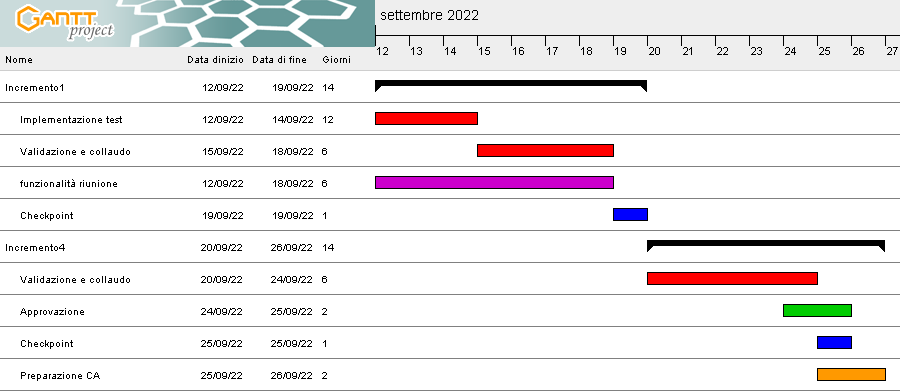
\includegraphics[width=\linewidth]{images/CA.png}
    \caption{Diagramma di Gantt - Macrofase CA}
\end{figure}
\newpage
\section{Preventivo}
      In questa sezione si riportano i preventivi per le varie fasi di lavoro elencate nel capitolo precedente. \newline
Si ricorda che il progetto didattico impone il vincolo che tutti i membri del gruppo ricoprino tutti i ruoli in modo equo.
Il gruppo rispetterà il vincolo nel progetto complessivo e non nelle singole fasi, 
altrimenti non si riuscirà a dare continuità al ruolo terminando i task assegnati.

\subsection{RTB}
\subsubsection{Baseline documentale}
\paragraph{Prospetto orario}
\begin{center}
	\renewcommand{\arraystretch}{1.8} %aumento ampiezza righe
	\begin{tabular}{ |m{10em}|c|c|c|c|c|c|c| }
	\hline
	\textbf{Membro} & \textbf{Re} & \textbf{Am} &  \textbf{An} &  \textbf{Pt} &  \textbf{Pg} &  \textbf{Ve} &  \textbf{Totale}\\
    \hline
    Irene Benetazzo   & 3 & - & 3 & - & - & - & \textbf{6} \\
    \hline
    Tommaso Berlaffa  & - & 5 & - & - & - & 1 & \textbf{6} \\
    \hline
    Mattia Episcopo   & - & 6 & - & - & - & - & \textbf{6} \\
    \hline
    Pietro Macrì      & - & 5 & - & - & - & 2 & \textbf{7} \\
    \hline
    Qi Fan Andrea Pan & - & 4 & 3 & - & - & - & \textbf{7} \\
    \hline
    Matteo Pillon     & - & 7 & - & - & - & - & \textbf{7} \\
    \hline
    Samuele Rizzato   & - & 4 & 3 & - & - & - & \textbf{7} \\
    \hline
    \textbf{Totale ore} & \textbf{3} & \textbf{31} &  \textbf{9} &  \textbf{0} &  \textbf{0} &  \textbf{3} &  \textbf{46}\\
    \hline
	\end{tabular}
\end{center}
\begin{figure}[H]
    \centering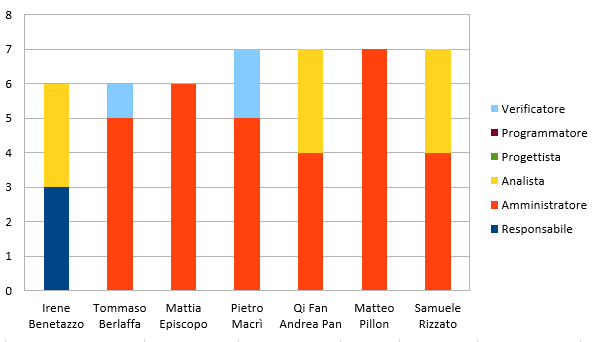
\includegraphics[width=\textwidth, height=\textheight, keepaspectratio]{images/preventivo/RTB-documentale-ore.png}
    \caption{RTB-Baseline documentale - preventivo ripartizione oraria}
\end{figure}


\paragraph{Prospetto economico}
\begin{center}
	\renewcommand{\arraystretch}{1.8} %aumento ampiezza righe
	\begin{tabular}{ |m{10em}|c|c|c|c|c|c|c| }
	\hline
	\textbf{Ruolo} & \textbf{Re} & \textbf{Am} &  \textbf{An} &  \textbf{Pt} &  \textbf{Pg} &  \textbf{Ve} &  \textbf{Totale}\\
    \hline
    Totale ore & 3 & 31 & 9 & 0 & 0 & 3 & \textbf{46}\\
    \hline
    Costo \euro/h & 30\euro/h & 20\euro/h & 25\euro/h & 25\euro/h & 15\euro/h & 15\euro/h & \\
    \hline
    \textbf{Totale costo} & \textbf{90\euro} & \textbf{620\euro} &  \textbf{225\euro} &  \textbf{0\euro} &  \textbf{0\euro} &  \textbf{45\euro} &  \textbf{980\euro}\\
    \hline
	\end{tabular}

    \begin{figure}[H]
        \centering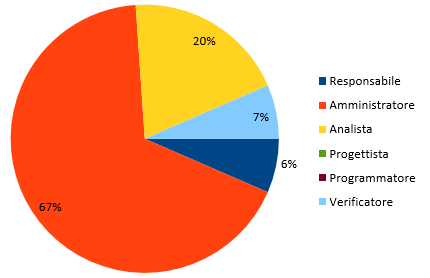
\includegraphics[width=0.7\textwidth, height=0.7\textheight, keepaspectratio]{images/preventivo/RTB-documentale-costo.png}
        \caption{RTB-Baseline documentale - preventivo ripartizione economica}
    \end{figure}
\end{center}


\subsubsection{Baseline dei requisiti}
\paragraph{Prospetto orario}
\begin{center}
	\renewcommand{\arraystretch}{1.8} %aumento ampiezza righe
	\begin{tabular}{ |m{10em}|c|c|c|c|c|c|c| }
	\hline
	\textbf{Membro} & \textbf{Re} & \textbf{Am} &  \textbf{An} &  \textbf{Pt} &  \textbf{Pg} &  \textbf{Ve} &  \textbf{Totale}\\
    \hline
    Irene Benetazzo   & - & 3 & 11 & - & - & 2 & \textbf{16} \\
    \hline
    Tommaso Berlaffa  & - & 1 & 13 & - & - & - & \textbf{14} \\
    \hline
    Mattia Episcopo   & - & 2 & 11 & - & - & - & \textbf{13} \\
    \hline
    Pietro Macrì      & - & 1 & 13 & - & - & - & \textbf{14} \\
    \hline
    Qi Fan Andrea Pan & - & 1 & 12 & - & - & - & \textbf{13} \\
    \hline
    Matteo Pillon     & - & 1 & 13 & - & - & 2 & \textbf{16} \\
    \hline
    Samuele Rizzato   & 3 & 1 & 11 & - & - & - & \textbf{15} \\
    \hline
    \textbf{Totale ore} & \textbf{3} & \textbf{10} &  \textbf{84} &  \textbf{0} &  \textbf{0} &  \textbf{4} &  \textbf{101}\\
    \hline
	\end{tabular}
\end{center}
\begin{figure}[H]
    \centering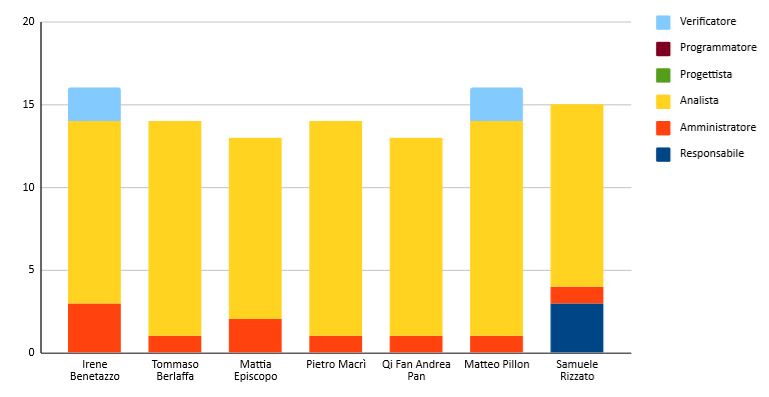
\includegraphics[width=\textwidth, height=\textheight,keepaspectratio]{images/preventivo/RTB-requisiti-ore.png}
    \caption{RTB-Baseline dei requisiti - preventivo ripartizione oraria}
\end{figure}

\paragraph{Prospetto economico}
\begin{center}
	\renewcommand{\arraystretch}{1.8} %aumento ampiezza righe
	\begin{tabular}{ |m{10em}|c|c|c|c|c|c|c| }
	\hline
	\textbf{Ruolo} & \textbf{Re} & \textbf{Am} &  \textbf{An} &  \textbf{Pt} &  \textbf{Pg} &  \textbf{Ve} &  \textbf{Totale}\\
    \hline
    Totale ore & 3 & 10 & 84 & 0 & 0 & 4 & \textbf{101}\\
    \hline
    Costo \euro/h & 30\euro/h & 20\euro/h & 25\euro/h & 25\euro/h & 15\euro/h & 15\euro/h & \\
    \hline
    \textbf{Totale costo} & \textbf{90\euro} & \textbf{200\euro} &  \textbf{2100\euro} &  \textbf{0\euro} &  \textbf{0\euro} &  \textbf{60\euro} &  \textbf{2450\euro}\\
    \hline
	\end{tabular}

    \begin{figure}[H]
        \centering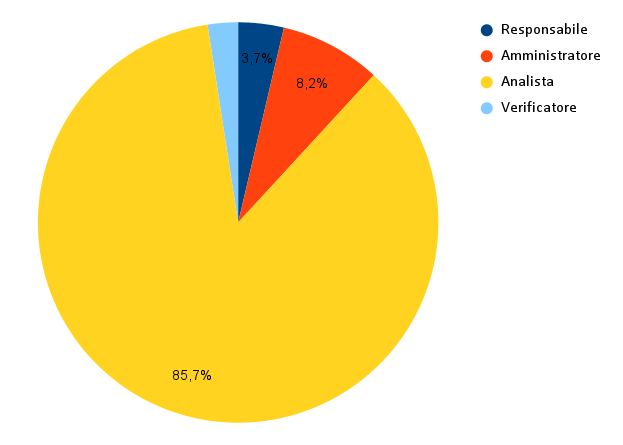
\includegraphics[width=0.7\textwidth, height=0.7\textheight, keepaspectratio]{images/preventivo/RTB-requisiti-costo.png}
        \caption{RTB-Baseline dei requisiti - preventivo ripartizione economica}
    \end{figure}
    
\end{center}

\subsubsection{Baseline delle tecnologie}
\paragraph{Prospetto orario}
\begin{center}
	\renewcommand{\arraystretch}{1.8} %aumento ampiezza righe
	\begin{tabular}{ |m{10em}|c|c|c|c|c|c|c| }
	\hline
	\textbf{Membro} & \textbf{Re} & \textbf{Am} &  \textbf{An} &  \textbf{Pt} &  \textbf{Pg} &  \textbf{Ve} &  \textbf{Totale}\\
    \hline
    Irene Benetazzo   & - & 8 & - & - & 2 & 2 & \textbf{12} \\
    \hline
    Tommaso Berlaffa  & - & - & - & 7 & 3 & 2 & \textbf{12} \\
    \hline
    Mattia Episcopo   & 1 & - & - & 8 & 3 & - & \textbf{12} \\
    \hline
    Pietro Macrì      & 1 & 1 & - & 7 & 3 & 0 & \textbf{12} \\
    \hline
    Qi Fan Andrea Pan & 3 & 2 & - & 4 & 3 & - & \textbf{12} \\
    \hline
    Matteo Pillon     & - & - & - & 7 & 3 & 2 & \textbf{12} \\
    \hline
    Samuele Rizzato   & 1 & 5 & 2 & - & 2 & 2 & \textbf{12} \\
    \hline
    \textbf{Totale ore} & \textbf{6} & \textbf{16} &  \textbf{2} &  \textbf{33} &  \textbf{19} &  \textbf{8} &  \textbf{84}\\
    \hline
	\end{tabular}
\end{center}
\begin{figure}[H]
    \centering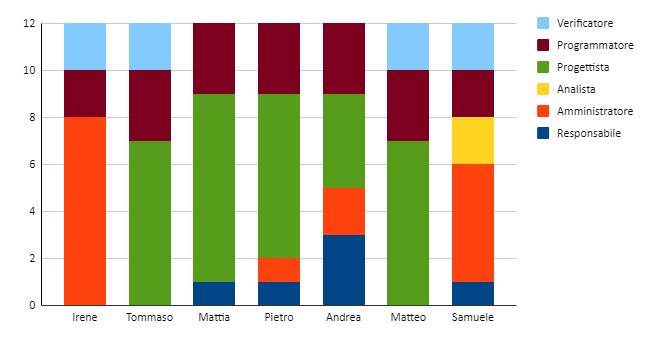
\includegraphics[width=\textwidth, height=\textheight,keepaspectratio]{images/preventivo/RTB-tecnologico-ore.png}
    \caption{RTB-Baseline delle tecnologie - preventivo ripartizione oraria}
\end{figure}

\paragraph{Prospetto economico}
\begin{center}
	\renewcommand{\arraystretch}{1.8} %aumento ampiezza righe
	\begin{tabular}{ |m{10em}|c|c|c|c|c|c|c| }
	\hline
	\textbf{Ruolo} & \textbf{Re} & \textbf{Am} &  \textbf{An} &  \textbf{Pt} &  \textbf{Pg} &  \textbf{Ve} &  \textbf{Totale}\\
    \hline
    Totale ore & 6 & 16 & 2 & 33 & 19 & 8 & \textbf{84}\\
    \hline
    Costo \euro/h & 30\euro/h & 20\euro/h & 25\euro/h & 25\euro/h & 15\euro/h & 15\euro/h & \\
    \hline
    \textbf{Totale costo} & \textbf{180\euro} & \textbf{320\euro} &  \textbf{50\euro} &  \textbf{825\euro} &  \textbf{285\euro} &  \textbf{120\euro} &  \textbf{1780\euro}\\
    \hline
	\end{tabular}

    \begin{figure}[H]
        \centering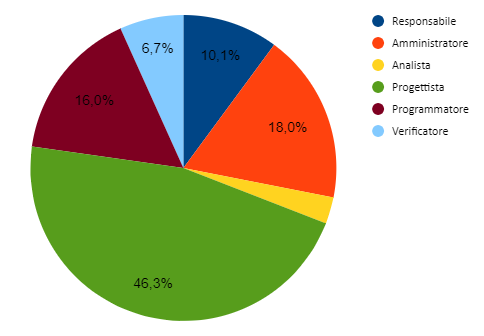
\includegraphics[width=0.7\textwidth, height=0.7\textheight, keepaspectratio]{images/preventivo/RTB-tecnologico-costo.png}
        \caption{RTB-Baseline delle tecnologie - preventivo ripartizione economica}
    \end{figure}
    
\end{center}

\newpage
      \subsection{PB}
Il preventivo di questa macrofase è stato stilato durante la precedente fase "baseline delle tecnologie" (della macrofase RTB) considerando anche i risparmi iniziali e rivalutando la ripartizione iniziale delle ore nei vari ruoli (scritte nel documento \emph{Candidatura.pdf}), per i dettagli sulla nuova ripartizione delle ore si legga la sezione \$6.1.4.4.
\subsubsection{Requisiti Obbligatori}
\paragraph{Incremento 1}
\subparagraph{Prospetto orario}
\begin{center}
	\renewcommand{\arraystretch}{1.8} %aumento ampiezza righe
	\begin{tabular}{ |m{10em}|c|c|c|c|c|c|c| }
	\hline
	\textbf{Membro} & \textbf{Re} & \textbf{Am} &  \textbf{An} &  \textbf{Pt} &  \textbf{Pg} &  \textbf{Ve} &  \textbf{Totale}\\
    \hline
    Irene Benetazzo   & - & - & - & 8 & 5 & 3 & \textbf{16} \\
    \hline
    Tommaso Berlaffa  & 3 & - & - & - & 10 & - & \textbf{13} \\
    \hline
    Mattia Episcopo   & - & 4 & - & 7 & 4 & 2 & \textbf{17} \\
    \hline
    Pietro Macrì      & - & 4 & - & 5 & 7 & 2 & \textbf{18} \\
    \hline
    Qi Fan Andrea Pan & - & - & - & 7 & 7 & 3 & \textbf{17} \\
    \hline
    Matteo Pillon     & - & - & - & 5 & 8 & 3 & \textbf{16} \\
    \hline
    Samuele Rizzato   & - & - & - & 8 & 5 & 3 & \textbf{16} \\
    \hline
    \textbf{Totale ore} & \textbf{3} & \textbf{8} &  \textbf{0} &  \textbf{40} &  \textbf{46} &  \textbf{16} &  \textbf{113}\\
    \hline
	\end{tabular}
\end{center}
\begin{figure}[H]
   \centering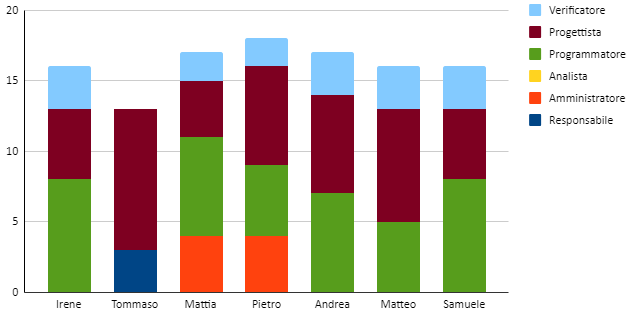
\includegraphics{images/preventivo/PB-incremento1-ore.png}
\end{figure}


\subparagraph{Prospetto economico}
\begin{center}
	\renewcommand{\arraystretch}{1.8} %aumento ampiezza righe
	\begin{tabular}{ |m{10em}|c|c|c|c|c|c|c| }
	\hline
	\textbf{Ruolo} & \textbf{Re} & \textbf{Am} &  \textbf{An} &  \textbf{Pt} &  \textbf{Pg} &  \textbf{Ve} &  \textbf{Totale}\\
    \hline
    Totale ore & 3 & 8 & 0 & 40 & 46 & 16 & \textbf{113}\\
    \hline
    Costo \euro/h & 30\euro/h & 20\euro/h & 25\euro/h & 25\euro/h & 15\euro/h & 15\euro/h & \\
    \hline
    \textbf{Totale costo} & \textbf{90\euro} & \textbf{160\euro} &  \textbf{0\euro} &  \textbf{1000\euro} &  \textbf{690\euro} &  \textbf{240\euro} &  \textbf{2180\euro}\\
    \hline
	\end{tabular}

    \begin{figure}[H]
       \centering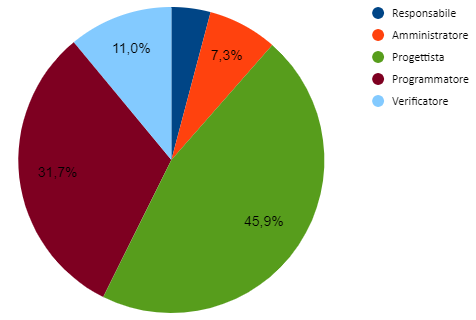
\includegraphics{images/preventivo/PB-incremento1-costo.png}
    \end{figure}
\end{center}



\paragraph{Incremento 2}
\subparagraph{Prospetto orario}
\begin{center}
	\renewcommand{\arraystretch}{1.8} %aumento ampiezza righe
	\begin{tabular}{ |m{10em}|c|c|c|c|c|c|c| }
	\hline
	\textbf{Membro} & \textbf{Re} & \textbf{Am} &  \textbf{An} &  \textbf{Pt} &  \textbf{Pg} &  \textbf{Ve} &  \textbf{Totale}\\
    \hline
    Irene Benetazzo   & - & - & - & 7 & 5 & 3 & \textbf{15} \\
    \hline
    Tommaso Berlaffa  & - & - & - & 6 & 6 & 3 & \textbf{15} \\
    \hline
    Mattia Episcopo   & 3 & - & - & - & 10 & - & \textbf{13} \\
    \hline
    Pietro Macrì      & - & - & - & 5 & 6 & 3 & \textbf{14} \\
    \hline
    Qi Fan Andrea Pan & - & 4 & - & 4 & 8 & 2 & \textbf{18} \\
    \hline
    Matteo Pillon     & - & - & - & 6 & 7 & 3 & \textbf{16} \\
    \hline
    Samuele Rizzato   & - & 5 & - & 6 & 5 & 3 & \textbf{19} \\
    \hline
    \textbf{Totale ore} & \textbf{3} & \textbf{9} &  \textbf{0} &  \textbf{34} &  \textbf{47} &  \textbf{17} &  \textbf{110}\\
    \hline
	\end{tabular}
\end{center}
\begin{figure}[H]
   \centering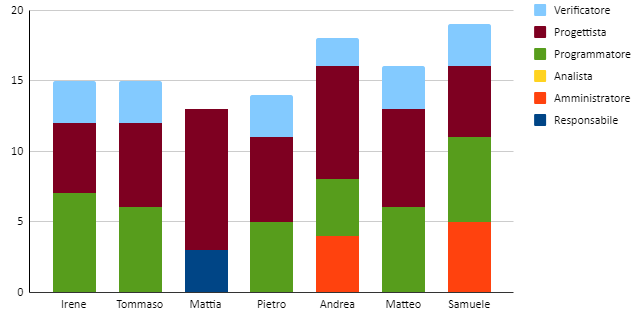
\includegraphics{images/preventivo/PB-incremento2-ore.png}
\end{figure}

\subparagraph{Prospetto economico}
\begin{center}
	\renewcommand{\arraystretch}{1.8} %aumento ampiezza righe
	\begin{tabular}{ |m{10em}|c|c|c|c|c|c|c| }
	\hline
	\textbf{Ruolo} & \textbf{Re} & \textbf{Am} &  \textbf{An} &  \textbf{Pt} &  \textbf{Pg} &  \textbf{Ve} &  \textbf{Totale}\\
    \hline
    Totale ore & 3 & 9 & 0 & 34 & 47 & 17 & \textbf{110}\\
    \hline
    Costo \euro/h & 30\euro/h & 20\euro/h & 25\euro/h & 25\euro/h & 15\euro/h & 15\euro/h & \\
    \hline
    \textbf{Totale costo} & \textbf{90\euro} & \textbf{180\euro} &  \textbf{0\euro} &  \textbf{1190\euro} &  \textbf{705\euro} &  \textbf{255\euro} &  \textbf{2420\euro}\\
    \hline
	\end{tabular}

    \begin{figure}[H]
       \centering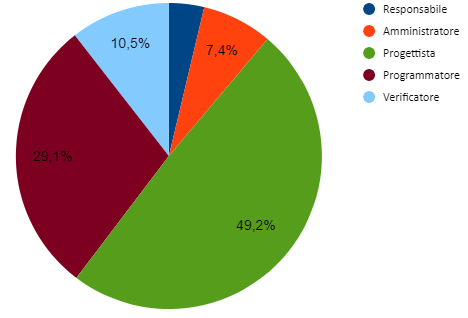
\includegraphics{images/preventivo/PB-incremento2-costo.png}
    \end{figure}
\end{center}


\subsubsection{Requisiti Desiderabili}
\paragraph{Incremento 3}
\subparagraph{Prospetto orario}
\begin{center}
	\renewcommand{\arraystretch}{1.8} %aumento ampiezza righe
	\begin{tabular}{ |m{10em}|c|c|c|c|c|c|c| }
	\hline
	\textbf{Membro} & \textbf{Re} & \textbf{Am} &  \textbf{An} &  \textbf{Pt} &  \textbf{Pg} &  \textbf{Ve} &  \textbf{Totale}\\
    \hline
    Irene Benetazzo   & - & - & - & 4 & 5 & 3 & \textbf{12} \\
    \hline
    Tommaso Berlaffa  & - & - & - & 5 & 4 & 3 & \textbf{12} \\
    \hline
    Mattia Episcopo   & - & 5 & - & 3 & 5 & 2 & \textbf{15} \\
    \hline
    Pietro Macrì      & 3 & - & - & - & 7 & - & \textbf{10} \\
    \hline
    Qi Fan Andrea Pan & - & - & - & 4 & 5 & 3 & \textbf{12} \\
    \hline
    Matteo Pillon     & - & 4 & - & 5 & 3 & 2 & \textbf{14} \\
    \hline
    Samuele Rizzato   & - & - & - & 5 & 5 & 3 & \textbf{13} \\
    \hline
    \textbf{Totale ore} & \textbf{3} & \textbf{9} &  \textbf{0} &  \textbf{26} &  \textbf{34} &  \textbf{16} &  \textbf{88}\\
    \hline
	\end{tabular}
\end{center}
\begin{figure}[H]
   \centering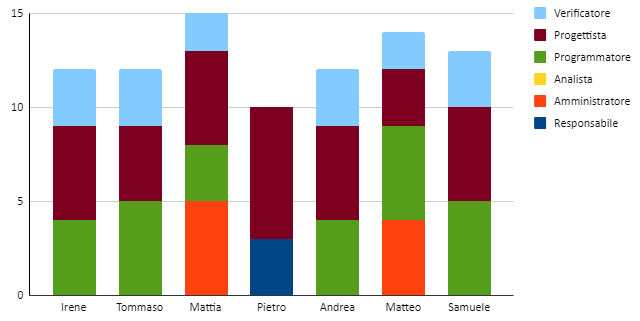
\includegraphics{images/preventivo/PB-incremento3-ore.png}
\end{figure}


\subparagraph{Prospetto economico}
\begin{center}
	\renewcommand{\arraystretch}{1.8} %aumento ampiezza righe
	\begin{tabular}{ |m{10em}|c|c|c|c|c|c|c| }
	\hline
    Totale ore & 3 & 9 & 0 & 26 & 34 & 16 & \textbf{88}\\
    \hline
    Costo \euro/h & 30\euro/h & 20\euro/h & 25\euro/h & 25\euro/h & 15\euro/h & 15\euro/h & \\
    \hline
    \textbf{Totale costo} & \textbf{90\euro} & \textbf{180\euro} &  \textbf{0\euro} &  \textbf{650\euro} &  \textbf{510\euro} &  \textbf{240\euro} &  \textbf{1730\euro}\\
    \hline
	\end{tabular}

    \begin{figure}[H]
       \centering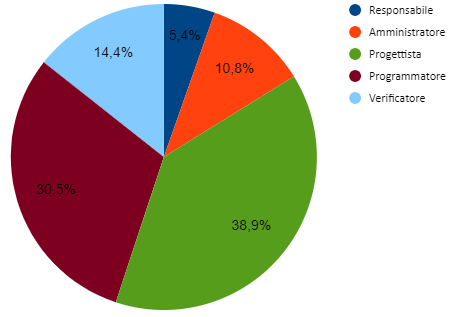
\includegraphics{images/preventivo/PB-incremento3-costo.png}
    \end{figure}
\end{center}



\paragraph{Incremento 4}
\subparagraph{Prospetto orario}
\begin{center}
	\renewcommand{\arraystretch}{1.8} %aumento ampiezza righe
	\begin{tabular}{ |m{10em}|c|c|c|c|c|c|c| }
	\hline
	\textbf{Membro} & \textbf{Re} & \textbf{Am} &  \textbf{An} &  \textbf{Pt} &  \textbf{Pg} &  \textbf{Ve} &  \textbf{Totale}\\
    \hline
    Irene Benetazzo   & - & 5 & - & 4 & 4 & 2 & \textbf{15} \\
    \hline
    Tommaso Berlaffa  & 1 & 4 & - & 4 & 4 & 3 & \textbf{16} \\
    \hline
    Mattia Episcopo   & 1 & - & - & 5 & 4 & 3 & \textbf{13} \\
    \hline
    Pietro Macrì      & 1 & - & - & 6 & 5 & 3 & \textbf{15} \\
    \hline
    Qi Fan Andrea Pan & 1 & - & - & 4 & 5 & 3 & \textbf{13} \\
    \hline
    Matteo Pillon     & 3 & 2 & - & - & 7 & - & \textbf{12} \\
    \hline
    Samuele Rizzato   & 1 & - & - & 4 & 5 & 3 & \textbf{13} \\
    \hline
    \textbf{Totale ore} & \textbf{8} & \textbf{11} &  \textbf{0} &  \textbf{27} &  \textbf{34} &  \textbf{17} &  \textbf{97}\\
    \hline
	\end{tabular}
\end{center}
\begin{figure}[H]
   \centering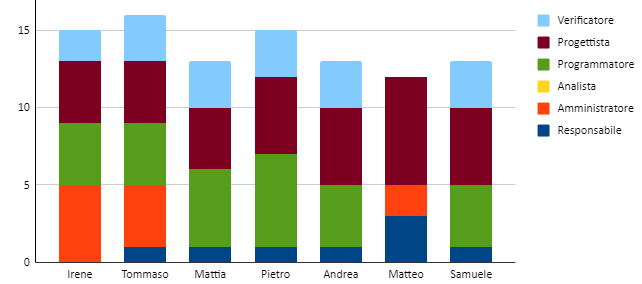
\includegraphics{images/preventivo/PB-incremento4-ore.png}
\end{figure}


\subparagraph{Prospetto economico}
\begin{center}
	\renewcommand{\arraystretch}{1.8} %aumento ampiezza righe
	\begin{tabular}{ |m{10em}|c|c|c|c|c|c|c| }
	\hline
	\textbf{Ruolo} & \textbf{Re} & \textbf{Am} &  \textbf{An} &  \textbf{Pt} &  \textbf{Pg} &  \textbf{Ve} &  \textbf{Totale}\\
    \hline
    Totale ore & 8 & 11 & 0 & 27 & 34 & 17 & \textbf{97}\\
    \hline
    Costo \euro/h & 30\euro/h & 20\euro/h & 25\euro/h & 25\euro/h & 15\euro/h & 15\euro/h & \\
    \hline
    \textbf{Totale costo} & \textbf{240\euro} & \textbf{220\euro} &  \textbf{0\euro} &  \textbf{675\euro} &  \textbf{510\euro} &  \textbf{255\euro} &  \textbf{1900\euro}\\
    \hline
	\end{tabular}

    \begin{figure}[H]
       \centering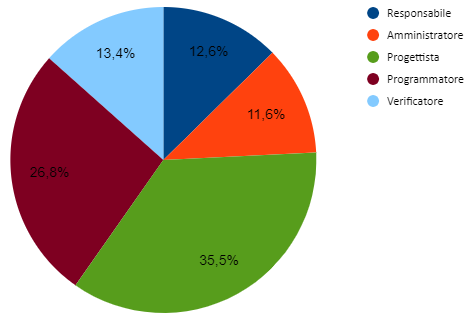
\includegraphics{images/preventivo/PB-incremento4-costo.png}
    \end{figure}
\end{center}

\newpage
      \subsection{CA}
Il preventivo della macrofase Customer Acceptance è stato stilato insieme alla decisione del preventivo a finire al termine della macrofase PB riportato alla sezione \$6.2.5.4
\subsubsection{Validazione requisiti obbligatori}
\paragraph{Prospetto Orario}
\begin{center}
	\renewcommand{\arraystretch}{1.8} %aumento ampiezza righe
	\begin{tabular}{ |m{10em}|c|c|c|c|c|c|c| }
	\hline
	\textbf{Membro} & \textbf{Re} & \textbf{Am} &  \textbf{An} &  \textbf{Pt} &  \textbf{Pg} &  \textbf{Ve} &  \textbf{Totale}\\
    \hline
    Irene Benetazzo   & - & 1 & - & 1 & - & 5 & \textbf{7} \\
    \hline
    Tommaso Berlaffa  & - & - & - & 2 & 2 & 3 & \textbf{7} \\
    \hline
    Mattia Episcopo   & - & - & - & - & 2 & 5 & \textbf{7} \\
    \hline
    Pietro Macrì      & - & - & - & 1 & 1 & 6 & \textbf{8} \\
    \hline
    Qi Fan Andrea Pan & - & 1 & - & - & 1 & 5 & \textbf{7} \\
    \hline
    Matteo Pillon     & - & - & - & 2 & - & 6 & \textbf{8} \\
    \hline
    Samuele Rizzato   & 2 & 2 & - & - & - & 2 & \textbf{6} \\
    \hline
    \textbf{Totale ore} & \textbf{2} & \textbf{4} &  \textbf{0} &  \textbf{6} &  \textbf{6} &  \textbf{32} &  \textbf{50}\\
    \hline
	\end{tabular}
\end{center}
\begin{figure}[H]
    \centering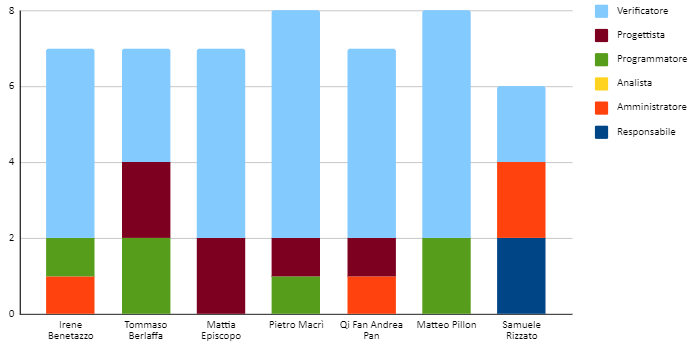
\includegraphics[width=\textwidth, height=\textheight, keepaspectratio]{images/preventivo/CA-obbligatori-orario.png}
    \caption{CA-validazione requisiti obbligatori - preventivo ripartizione oraria}
\end{figure}

\paragraph{Prospetto Economico}
\begin{center}
	\renewcommand{\arraystretch}{1.8} %aumento ampiezza righe
	\begin{tabular}{ |m{10em}|c|c|c|c|c|c|c| }
	\hline
	\textbf{Ruolo} & \textbf{Re} & \textbf{Am} &  \textbf{An} &  \textbf{Pt} &  \textbf{Pg} &  \textbf{Ve} &  \textbf{Totale}\\
    \hline
    Totale ore & 2 & 4 & 0 & 6 & 6 & 32 & \textbf{50}\\
    \hline
    Costo \euro/h & 30\euro/h & 20\euro/h & 25\euro/h & 25\euro/h & 15\euro/h & 15\euro/h & \\
    \hline
    \textbf{Totale costo} & \textbf{60\euro} & \textbf{80\euro} &  \textbf{0\euro} &  \textbf{150\euro} &  \textbf{90\euro} &  \textbf{480\euro} &  \textbf{860\euro}\\
    \hline
	\end{tabular}

\begin{figure}[H]
    \centering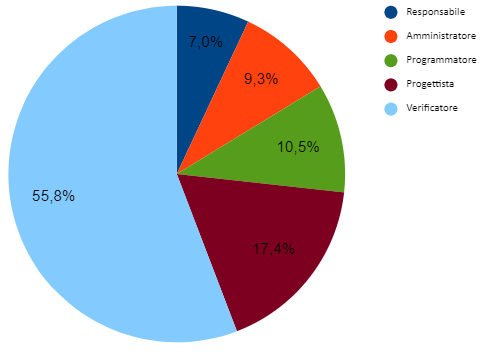
\includegraphics[scale=0.9]{images/preventivo/CA-obbligatori-costo.png}
    \caption{CA-validazione requisiti obbligatori - preventivo ripartizione economica}
\end{figure}
\end{center}

\newpage
\subsubsection{Validazione requisiti desiderabili}
\paragraph{Prospetto Orario}
\begin{center}
	\renewcommand{\arraystretch}{1.8} %aumento ampiezza righe
	\begin{tabular}{ |m{10em}|c|c|c|c|c|c|c| }
	\hline
	\textbf{Membro} & \textbf{Re} & \textbf{Am} &  \textbf{An} &  \textbf{Pt} &  \textbf{Pg} &  \textbf{Ve} &  \textbf{Totale}\\
    \hline
    Irene Benetazzo   & 2 & 2 & - & - & - & 3 & \textbf{7} \\
    \hline
    Tommaso Berlaffa  & - & 2 & - & - & - & 6 & \textbf{8} \\
    \hline
    Mattia Episcopo   & 1 & - & - & - & - & 4 & \textbf{5} \\
    \hline
    Pietro Macrì      & - & 2 & - & - & 2 & 5 & \textbf{9} \\
    \hline
    Qi Fan Andrea Pan & - & - & - & 3 & - & 6 & \textbf{9} \\
    \hline
    Matteo Pillon     & - & - & - & - & 1 & 5 & \textbf{6} \\
    \hline
    Samuele Rizzato   & - & - & - & 1 & 1 & 4 & \textbf{6} \\
    \hline
    \textbf{Totale ore} & \textbf{3} & \textbf{6} &  \textbf{0} &  \textbf{4} &  \textbf{4} &  \textbf{33} &  \textbf{50}\\
    \hline
	\end{tabular}
\end{center}
\begin{figure}[H]
    \centering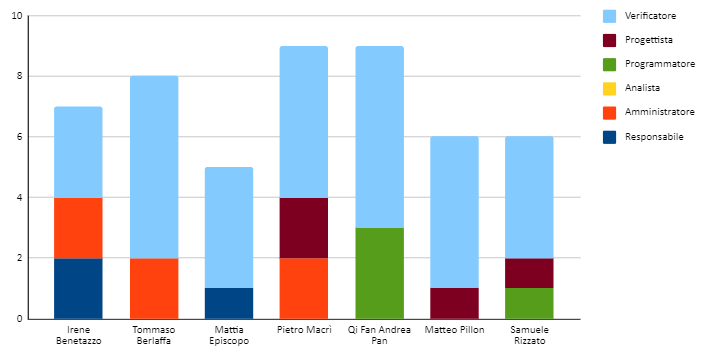
\includegraphics[width=\textwidth, height=\textheight, keepaspectratio]{images/preventivo/CA-desiderabili-orario.png}
    \caption{CA-validazione requisiti desiderabili - preventivo ripartizione oraria}
\end{figure}
\pagebreak
\paragraph{Prospetto Economico}
\begin{center}
	\renewcommand{\arraystretch}{1.8} %aumento ampiezza righe
	\begin{tabular}{ |m{10em}|c|c|c|c|c|c|c| }
	\hline
	\textbf{Ruolo} & \textbf{Re} & \textbf{Am} &  \textbf{An} &  \textbf{Pt} &  \textbf{Pg} &  \textbf{Ve} &  \textbf{Totale}\\
    \hline
    Totale ore & 3 & 6 & 0 & 4 & 4 & 33 & \textbf{50}\\
    \hline
    Costo \euro/h & 30\euro/h & 20\euro/h & 25\euro/h & 25\euro/h & 15\euro/h & 15\euro/h & \\
    \hline
    \textbf{Totale costo} & \textbf{90\euro} & \textbf{120\euro} &  \textbf{0\euro} &  \textbf{100\euro} &  \textbf{60\euro} &  \textbf{495\euro} &  \textbf{865\euro}\\
    \hline
	\end{tabular}

\begin{figure}[H]
    \centering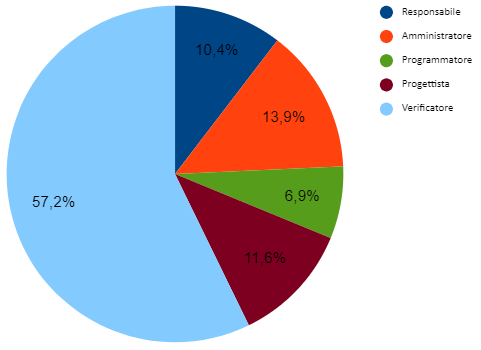
\includegraphics[scale=0.9]{images/preventivo/CA-desiderabili-costo.png}
    \caption{CA-validazione requisiti desiderabili - preventivo ripartizione economica}
\end{figure}
\end{center}


\newpage
\section{Consuntivo}
      In questa sezione si raccolgono le consuntivazioni orarie ed i reali costi delle varie fasi di lavoro elencate nel 
capitolo 4 e preventivate nel capitolo 5. \newline
Per ogni fase verranno scritti i seguenti punti, evidenziando le differenze rispetto al preventivo:
\begin{enumerate}
    \item consuntivo orario;
    \item consuntivo economico;
    \item considerazioni.
\end{enumerate}
In particolare nelle considerazioni si motiva l'eventuale scostamento notevole rispetto al preventivo
e di conseguenza potrebbe essere necessario rimaneggiare il preventivo delle fasi successive.
Il bilancio tra consuntivo e preventivo può essere:
\begin{itemize}
    \item \textbf{Negativo: } spesa minore rispetto al preventivo
    \item \textbf{Uguale: } nessuna differenza di spesa tra preventivo e consuntivo
    \item \textbf{Positivo: } spesa maggiore rispetto al preventivo
\end{itemize}
Per bilancio complessivo si intende sommare le differenze dei bilanci precedenti 
fino ad ottenere bilancio del momento.

\subsection{RTB}
\subsubsection{Baseline documentale}
\paragraph{Consuntivo orario}
\begin{center}
	\renewcommand{\arraystretch}{1.8} %aumento ampiezza righe
	\begin{tabular}{ |m{8em}|c|c|c|c|c|c|c| }
	\hline
	\textbf{Membro} & \textbf{Re} & \textbf{Am} &  \textbf{An} &  \textbf{Pt} &  \textbf{Pg} &  \textbf{Ve} &  \textbf{Totale}\\
    \hline
    Irene Benetazzo   & 4 (+1) & -      & 0 (-3) & - & - & -     & \textbf{4} (-2) \\
    \hline
    Tommaso Berlaffa  & -      & 3 (-2) & -      & - & - & 1      & \textbf{4} (-2) \\
    \hline
    Mattia Episcopo   & -      & 3 (-3) & 2 (+2) & - & - & -      & \textbf{5} (-1) \\
    \hline
    Pietro Macrì      & -      & 4 (-1) & -      & - & - & 1 (-1) & \textbf{5} (-2) \\
    \hline
    Qi Fan Andrea Pan & -      & 3 (-1) & 2 (-1) & - & - & -      & \textbf{5} (-2) \\
    \hline
    Matteo Pillon     & -      & 4 (-3) & -      & - & - & -      & \textbf{4} (-3) \\
    \hline
    Samuele Rizzato   & -      & 3 (-1) & 2 (-1) & - & - & -      & \textbf{5} (-2) \\
    \hline
    \textbf{Totale ore} & \textbf{4} (+1) & \textbf{20} (-11) &  \textbf{6} (-3) &  \textbf{0} &  \textbf{0} &  \textbf{2} (-1) &  \textbf{32} (-14)\\
    \hline
	\end{tabular}
\end{center}
\begin{figure}[H]
    \centering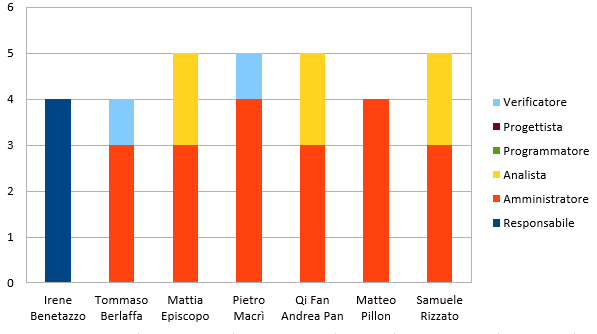
\includegraphics{images/consuntivo/RTB-documentale-ore.png}
\end{figure}

\paragraph{Consuntivo economico}
\begin{center}
	\renewcommand{\arraystretch}{1.8} %aumento ampiezza righe
	\begin{tabular}{ |m{6em}|c|c|c|c|c|c|c| }
	\hline
	\textbf{Ruolo} & \textbf{Re} & \textbf{Am} &  \textbf{An} &  \textbf{Pt} &  \textbf{Pg} &  \textbf{Ve} &  \textbf{Totale}\\
    \hline
    Totale ore & 4 & 20 & 6 & 0 & 0 & 2 & \textbf{32}\\
    \hline
    Costo \euro/h & 30\euro/h & 20\euro/h & 25\euro/h & 25\euro/h & 15\euro/h & 15\euro/h & \\
    \hline
    \textbf{Totale costo} & \textbf{120\euro} & \textbf{400\euro} &  \textbf{150\euro} & \textbf{0\euro} &  \textbf{0\euro} &  \textbf{30\euro} &  \textbf{700\euro} \\
    & (+30\euro) & (-120\euro) & (-75\euro) &  &  & (-15\euro) & (-280\euro) \\
    \hline
	\end{tabular}

    \begin{figure}[H]
       \centering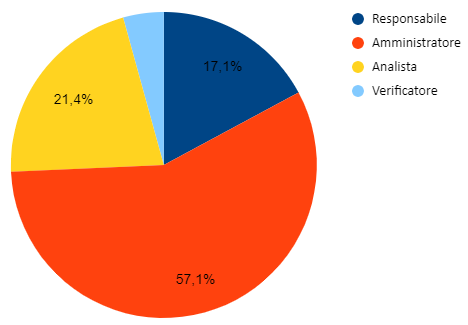
\includegraphics[width=0.6\textwidth, height=0.6\textheight, keepaspectratio]{images/consuntivo/RTB-documentale-costo.png}
    \end{figure}
\end{center}

\paragraph{Considerazioni} \hfill \break
Erano state preventivate più ore (e giorni) di lavoro per gli amministratori, dato il cospicuo 
numero di pagine dei documenti e si pensava fosse necessario più studio anche per gli analisti.
Quindi questa fase si chiude 7 giorni prima del previsto cioè il 26 Aprile, con un risparmio di 280\euro. 
\begin{center}
	\renewcommand{\arraystretch}{1.8} %aumento ampiezza righe
	\begin{tabular}{ | l |c|c| }
    \hline
    & \textbf{Ore} & \textbf{Costo} \\
	\hline
    \textbf{Consuntivo} & 32 & 700\euro \\
    \hline
    \textbf{Preventivo} & 46 & 980\euro \\
    \hline
    \textbf{Bilancio fase} & -14 & -280\euro \\
    \hline
    \textbf{Bilancio complessivo} & \textbf{-14} & \textbf{-280\euro} \\
    \hline
    \end{tabular}
\end{center}

Di conseguenza si decide di partire subito con la fase successiva: Baseline dei Requisiti di cui inizialmente 
è stata prevista una sola settimana di lavoro, ma dato la grande mole di casi d'uso da identificare e 
analizzare nel progetto probabilmente verrà usato parte del risparmio di questa fase.

\subsubsection{Baseline dei requisiti}
\paragraph{Consuntivo orario}
\begin{center}
	\renewcommand{\arraystretch}{1.8}
	\begin{tabular}{ |c|c|c|c|c|c|c|c| }
	\hline
	\textbf{Membro} & \textbf{Re} & \textbf{Am} &  \textbf{An} &  \textbf{Pt} &  \textbf{Pg} &  \textbf{Ve} &  \textbf{Totale}\\
    \hline
    Irene Benetazzo   & - & 3      & 6  (-5) & - & - & 2 & \textbf{11} (-5) \\
    \hline
    Tommaso Berlaffa  & - & 1      & 13      & - & - & - & \textbf{14}      \\
    \hline
    Mattia Episcopo   & - & - (-2) & 13 (+2) & - & - & - & \textbf{13}      \\
    \hline
    Pietro Macrì      & - & 1      & 7  (-6) & - & - & - & \textbf{8} (-6)  \\
    \hline
    Qi Fan Andrea Pan & - & 1      & 7  (-5) & - & - & - & \textbf{8} (-5)  \\
    \hline
    Matteo Pillon     & - & - (-1) & 11 (-2) & - & - & 2 & \textbf{13} (-3) \\
    \hline
    Samuele Rizzato   & 3 & 1      & 5  (-6) & - & - & - & \textbf{9} (-6)  \\
    \hline
    \textbf{Totale ore} & \textbf{3} & \textbf{7} (-3) &  \textbf{62} (-22) &  \textbf{0} &  \textbf{0} &  \textbf{4} &  \textbf{76} (-25)\\
    \hline
	\end{tabular}
\end{center}
\begin{figure}[H]
    \centering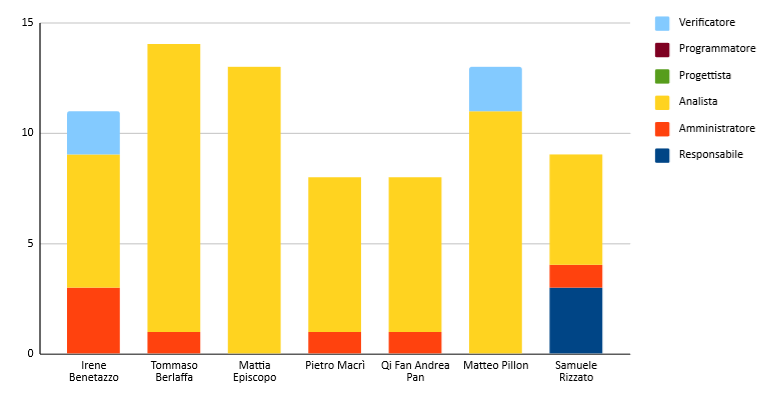
\includegraphics[width=\textwidth, height=\textheight,keepaspectratio]{images/consuntivo/RTB-requisiti-ore.png}
\end{figure}

\paragraph{Consuntivo economico}
\begin{center}
	\renewcommand{\arraystretch}{1.8}
	\begin{tabular}{ |m{6em}|c|c|c|c|c|c|c| }
	\hline
	\textbf{Ruolo} & \textbf{Re} & \textbf{Am} &  \textbf{An} &  \textbf{Pt} &  \textbf{Pg} &  \textbf{Ve} &  \textbf{Totale}\\
    \hline
    Totale ore & 3 & 7 & 62 & 0 & 0 & 4 & \textbf{76}\\
    \hline
    Costo \euro/h & 30\euro/h & 20\euro/h & 25\euro/h & 25\euro/h & 15\euro/h & 15\euro/h & \\
    \hline
    \textbf{Totale costo} & \textbf{90\euro} & \textbf{140\euro} &  \textbf{1550\euro} & \textbf{0\euro} &  \textbf{0\euro} &  \textbf{60\euro} &  \textbf{1840\euro} \\
    &  & (-60\euro) & (-550\euro) &  &  &  & (-610\euro) \\
    \hline
	\end{tabular}

    \begin{figure}[H]
        \centering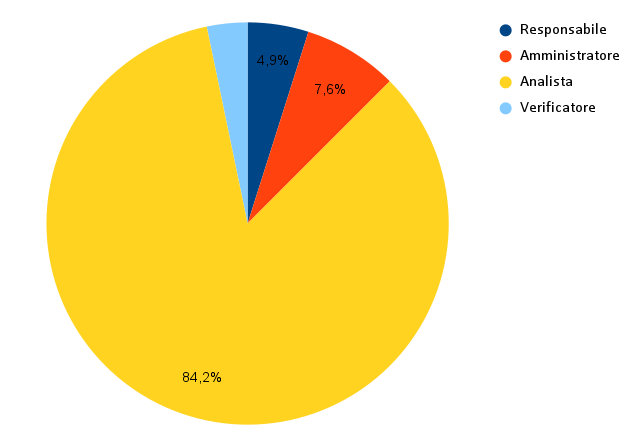
\includegraphics[width=0.7\textwidth, height=0.7\textheight, keepaspectratio]{images/consuntivo/RTB-requisiti-costo.png}
    \end{figure}
\end{center}

\paragraph{Considerazioni} \hfill \break
Per la maggior parte dei membri del gruppo sono state preventivate più ore di quelle necessarie come analisti in quanto 
si pensava che l'Analisi dei Requisiti avrebbe preso molto tempo per l'identificazione e lo studio dei casi d'uso, inoltre è stata
fatta una sovrastima delle ore da amministratore poiché il team si è dedicato di più all'Analisi dei Requisiti 
che all'aggiornamento dei vari documenti.

\begin{center}
	\renewcommand{\arraystretch}{1.8}
	\begin{tabular}{ | l |c|c| }
    \hline
    & \textbf{Ore} & \textbf{Costo} \\
	\hline
    \textbf{Consuntivo} & 76 & 1840\euro \\
    \hline
    \textbf{Preventivo} & 101 & 2450\euro \\
    \hline
    \textbf{Bilancio fase} & -25 & -610\euro \\
    \hline
    \textbf{Bilancio complessivo} & \textbf{-39} & \textbf{-890\euro} \\
    \hline
    \end{tabular}
\end{center}
In conclusione la fase Baseline dei Requisiti termina il 2022-05-09 come prestabilito con un risparmio, relativo
alla fase, di 610€.

\subsubsection{Baseline delle tecnologie}
\paragraph{Consuntivo orario}
\begin{center}
	\renewcommand{\arraystretch}{1.8}
	\begin{tabular}{ |c|c|c|c|c|c|c|c| }
	\hline
	\textbf{Membro} & \textbf{Re} & \textbf{Am} &  \textbf{An} &  \textbf{Pt} &  \textbf{Pg} &  \textbf{Ve} &  \textbf{Totale}\\
    \hline
    Irene Benetazzo   & - & 8 & - & - & 2 & 2 & \textbf{12} \\
    \hline
    Tommaso Berlaffa  & - & - & - & 7 & 3 & -(-2) & \textbf{10} \\
    \hline
    Mattia Episcopo   & 1 & - & - & 8 & 3 & - & \textbf{12} \\
    \hline
    Pietro Macrì      & 1 & 1 & - & 7 & 3 & 2(+2) & \textbf{14} \\
    \hline
    Qi Fan Andrea Pan & 3 & 2 & - & 4 & 3 & - & \textbf{12} \\
    \hline
    Matteo Pillon     & - & - & - & 7 & 3 & 2 & \textbf{12} \\
    \hline
    Samuele Rizzato   & 1 & 5 & 2 & - & 2 & 2 & \textbf{12} \\
    \hline
    \textbf{Totale ore} & \textbf{6} & \textbf{16} &  \textbf{2} &  \textbf{33} &  \textbf{19} &  \textbf{8} &  \textbf{84}\\
    \hline
	\end{tabular}
\end{center}
\begin{figure}[H]
    \centering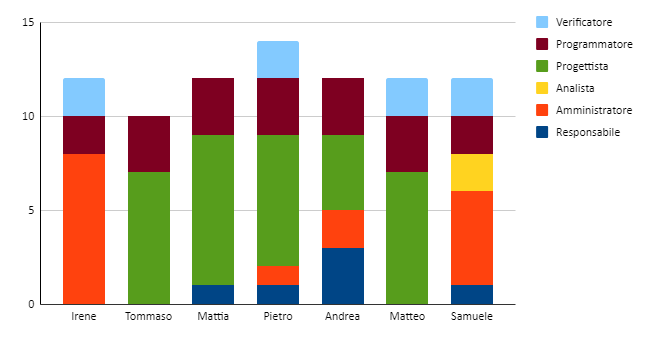
\includegraphics[width=\textwidth, height=\textheight,keepaspectratio]{images/consuntivo/RTB-tecnologico-ore.png}
\end{figure}

\paragraph{Consuntivo economico}
\begin{center}
	\renewcommand{\arraystretch}{1.8}
	\begin{tabular}{ |m{6em}|c|c|c|c|c|c|c| }
	\hline
	\textbf{Ruolo} & \textbf{Re} & \textbf{Am} &  \textbf{An} &  \textbf{Pt} &  \textbf{Pg} &  \textbf{Ve} &  \textbf{Totale}\\
    \hline
    Totale ore & 6 & 16 & 2 & 33 & 19 & 8 & \textbf{84}\\
    \hline
    Costo \euro/h & 30\euro/h & 20\euro/h & 25\euro/h & 25\euro/h & 15\euro/h & 15\euro/h & \\
    \hline
    \textbf{Totale costo} & \textbf{180\euro} & \textbf{320\euro} &  \textbf{50\euro} &  \textbf{825\euro} &  \textbf{285\euro} &  \textbf{120\euro} &  \textbf{1780\euro}\\
    \hline
	\end{tabular}
    \begin{figure}[H]
        \centering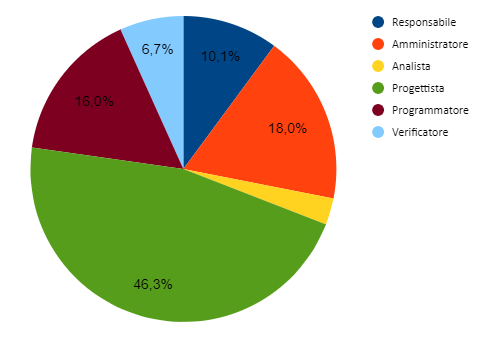
\includegraphics[width=0.7\textwidth, height=0.7\textheight, keepaspectratio]{images/consuntivo/RTB-tecnologico-costo.png}
    \end{figure}
\end{center}

\paragraph{Considerazioni} \hfill \break
Durante questa macrofase a livello economico è sono stati risparmiati o, anche se a livello temporale è stata necessaria una settimana in più.
Il motivo principale è stato lo studio delle tecnologie necessarie per il PoC, essendo nuove per i membri del gruppo, le ore di studio personale non sono state conteggiate. \newline
\begin{center}
	\renewcommand{\arraystretch}{1.8}
	\begin{tabular}{ | l |c|c| }
    \hline
    & \textbf{Ore} & \textbf{Costo} \\
	\hline
    \textbf{Consuntivo} & 84 & 1780\euro \\
    \hline
    \textbf{Preventivo} & 84 & 1780\euro \\
    \hline
    \textbf{Bilancio fase} & 0 & 0\euro \\
    \hline
    \textbf{Bilancio complessivo} & \textbf{-39} & \textbf{-890\euro} \\
    \hline
    \end{tabular}
\end{center}
In conclusione la fase Baseline delle Tecnologie termina il 2022-05-31.


\subsubsection{Complessivo RTB}
\paragraph{Consuntivo orario}
\begin{center}
	\renewcommand{\arraystretch}{1.8}
	\begin{tabular}{ |c|c|c|c|c|c|c|c| }
	\hline
	\textbf{Membro} & \textbf{Re} & \textbf{Am} &  \textbf{An} &  \textbf{Pt} &  \textbf{Pg} &  \textbf{Ve} &  \textbf{Totale}\\
    \hline
    Irene Benetazzo   & 4 & 11 & 6 & - & 2 & 4 & \textbf{27} \\
    \hline
    Tommaso Berlaffa  & - & 4 & 13 & 7 & 3 & 1 & \textbf{28} \\
    \hline
    Mattia Episcopo   & 1 & 3 & 15 & 8 & 3 & - & \textbf{30} \\
    \hline
    Pietro Macrì      & 1 & 6 & 7 & 7 & 3 & 3 & \textbf{27} \\
    \hline
    Qi Fan Andrea Pan & 3 & 6 & 9 & 4 & 3 & - & \textbf{25} \\
    \hline
    Matteo Pillon     & - & 4 & 11 & 7 & 3 & 4 & \textbf{29} \\
    \hline
    Samuele Rizzato   & 4 & 9 & 9 & - & 2 & 2 & \textbf{26} \\
    \hline
    \textbf{Totale ore} & \textbf{13} & \textbf{43} &  \textbf{70} &  \textbf{33} &  \textbf{19} &  \textbf{14} &  \textbf{192}\\
    \hline
	\end{tabular}
\end{center}
\begin{figure}[H]
    \centering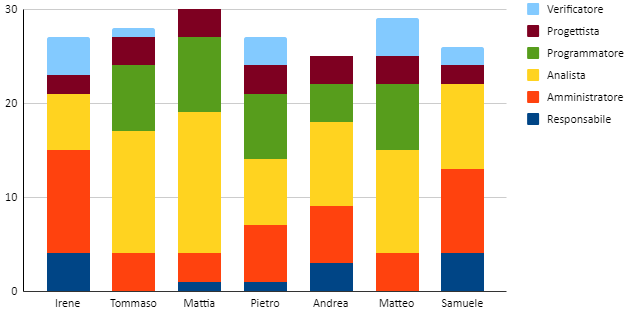
\includegraphics[width=\textwidth, height=\textheight,keepaspectratio]{images/consuntivo/RTB-ore.png}
\end{figure}

\paragraph{Consuntivo economico}
\begin{center}
	\renewcommand{\arraystretch}{1.8}
	\begin{tabular}{ |m{6em}|c|c|c|c|c|c|c| }
	\hline
	\textbf{Ruolo} & \textbf{Re} & \textbf{Am} &  \textbf{An} &  \textbf{Pt} &  \textbf{Pg} &  \textbf{Ve} &  \textbf{Totale}\\
    \hline
    Totale ore & 13 & 43 & 70 & 33 & 19 & 14 & \textbf{192}\\
    \hline
    Costo \euro/h & 30\euro/h & 20\euro/h & 25\euro/h & 25\euro/h & 15\euro/h & 15\euro/h & \\
    \hline
    \textbf{Totale costo} & \textbf{390\euro} & \textbf{860\euro} &  \textbf{1750\euro} &  \textbf{825\euro} &  \textbf{285\euro} &  \textbf{210\euro} &  \textbf{4320\euro}\\
    \hline
	\end{tabular}

    \begin{figure}[H]
        \centering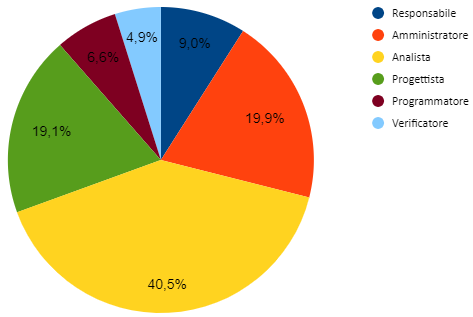
\includegraphics[width=0.7\textwidth, height=0.7\textheight, keepaspectratio]{images/consuntivo/RTB-costo.png}
    \end{figure}
\end{center}

\paragraph{Considerazioni} \hfill \break
\begin{center}
	\renewcommand{\arraystretch}{1.8}
	\begin{tabular}{ | l |c|c| }
    \hline
    & \textbf{Ore} & \textbf{Costo} \\
	\hline
    \textbf{Consuntivo} & 192 & 4320\euro \\
    \hline
    \textbf{Preventivo} & 231 & 5210\euro \\
    \hline
    \textbf{Bilancio} & \textbf{-39} & \textbf{-890\euro} \\
    \hline
    \end{tabular}
\end{center}
In conclusione la macrofase Requirements Tecnology Baseline iniziata il 2022-04-19 termina il 2022-06-01 con un ritardo di 9 giorni e un risparmio di 890\euro.

\paragraph{Preventivo a finire} \hfill \break
Considerato l'avanzo complessivo di 39 ore oltre ad una non corretta distribuzione delle ore nei specifici ruoli, nel documento \emph{Candidatura.pdf}, si è deciso di ridistribuire la pianificazione delle ore nei ruoli:
\begin{center}
	\renewcommand{\arraystretch}{1.8}
	\begin{tabular}{ | l |c|c|c| }
    \hline
    \textbf{Ruolo} & \textbf{Preventivo attuale} & \textbf{Preventivo iniziale}  & \textbf{Differenza economica}\\
	\hline
    \textbf{Responsabile} & 40 & 40 & 0\euro \\
    \hline
    \textbf{Amministratore} & 90 & 100 & -200\euro \\
    \hline
    \textbf{Analista} & 70 & 100 & -750\euro \\
    \hline
    \textbf{Progettista} & 170 & 160 & 250\euro \\
    \hline
    \textbf{Programmatore} & 190 & 160 & 450\euro \\
    \hline
    \textbf{Verificatore} & 140 & 140 & 0\euro \\
    \hline
    \textbf{Totale} & \textbf{700} & \textbf{700} & \textbf{-250\euro} \\
    \hline
    \end{tabular}
\end{center}
Non è cambiato il numero complessivo di ore ma la distribuzione interna e dato la differenza di prezzo tra i vari ruoli, ciò ha portato ad un risparmio di 250 \euro. \newline
Il preventivo della macrofase Product Baseline (\$5.2) è stato stilato basandosi sul preventivo attuale.
\end{document}